\documentclass[11pt]{article}

\usepackage[margin=1in]{geometry}
\usepackage{amsmath,amssymb,amsfonts}
\usepackage{graphicx}
\usepackage{booktabs}
\usepackage{hyperref}
\usepackage{siunitx}
\usepackage{enumitem}

\title{Influence Suppression and Consensus Cycling in Status-Penalized Networks}
\author{Advit Singh}
\date{September 2026}

\begin{document}
\maketitle

\begin{abstract}
Distributed consensus models usually treat communication weights as accuracy-seeking or static.
This paper introduces an asymmetric status-suppression operator that penalizes agents whose
estimates exceed the network mean, coupled with partial cognitive anchoring to initial private
values. The resulting closed-loop system is a switched affine opinion dynamics model whose
stability depends jointly on penalty severity, stubbornness, topology, and kinship structure.
A factorial simulation study over 368{,}991 validated runs identifies four stability regimes:
biased convergence, fixed dissensus, slow mixing, and non-convergent cycling. Cycling in the
proposed model is rare (0.02\%) and appears only under maximal suppression with non-zero
stubbornness, while symmetric suppression and inverse-variance baselines show very different
failure modes. Kinship clusters of size at least $N/5$ eliminate cycling across all tested
configurations.
\end{abstract}

\section{1. Introduction}
Distributed average-consensus algorithms formalize how decentralized networks of autonomous agents reach shared numerical agreements through local message passing\cite{degroot1974reaching}. In classical frameworks such as the DeGroot model, agents update their scalar estimates over discrete time steps through convex combinations of their neighbors' prior states\cite{degroot1974reaching}. Most extensions to this architecture assume that communication channels are static, unweighted, or adaptively weighted to prioritize accuracy, historical prestige, or metric proximity\cite{degroot1974reaching}. Under standard conditions of persistent connectivity and aperiodicity, these systems contract toward a static consensus lying strictly within the convex hull of initial network estimates\cite{degroot1974reaching}.

Empirical sociology and organizational psychology document a persistent counter-behavior in human collectives: groups frequently penalize their highest-performing members\cite{degroot1974reaching}. This behavioral tendency, formalized in social psychology as "tall poppy syndrome," describes the social derogation, exclusion, or sanctioning of individuals whose achievements or accuracy significantly surpass the group average\cite{degroot1974reaching}. While leveling mechanisms, reverse dominance hierarchies, and anti-outlier pressures are documented across varied institutional and cultural contexts, asymmetric status-based penalties targeting positive performance have been absent from mathematical opinion dynamics\cite{degroot1974reaching}.

This paper addresses that gap by introducing an endogenous, status-based weight suppression operator into a distributed consensus network\cite{degroot1974reaching}. The central question driving this work is operational: if an agent's outgoing broadcast influence is systematically reduced as a function of its positive deviation from the collective mean, does this leveling pressure impede or destabilize network consensus\cite{degroot1974reaching}? In estimation tasks where an outlier pulls the collective toward a ground truth, this mechanism penalizes the network's most informative agent precisely because of its accuracy\cite{degroot1974reaching}.

Analyzing this mechanism requires moving beyond linear systems theory\cite{degroot1974reaching}. Because influence weights vary at each discrete step based on instantaneous agent opinions, the interaction topology forms a closed-loop, state-dependent dynamical system\cite{degroot1974reaching,hajnal1958weak}. Previous treatments of time-varying consensus frequently rely on open-loop non-homogeneous Markov chain ergodicity, using Hajnal contraction coefficients to evaluate whether an exogenous sequence of stochastic matrices contracts to rank one\cite{degroot1974reaching,hajnal1958weak}. In the presence of cognitive anchoring, however, the governing difference equation is affine rather than linear\cite{acemoglu2013opinion,hajnal1958weak}. The network transition matrix remains strictly row-stochastic by construction, ensuring that estimates remain bounded within the convex hull of initial conditions and preventing numerical divergence\cite{degroot1974reaching}. The appropriate analytical framework is therefore the theory of switched affine systems and discrete-time bifurcations\cite{acemoglu2013opinion,hajnal1958weak}. The peer interaction operator acts as a contraction mapping on the disagreement subspace, while cognitive anchors continuously inject initial state dispersion back into the network\cite{acemoglu2013opinion,hajnal1958weak}.

This formulation introduces a cognitive resistance parameter: partial stubbornness ($\gamma_{stub} \in [0, 1)$)\cite{degroot1974reaching}. In a pure averaging update without cognitive memory ($\gamma_{stub} = 0$), an outlier whose outgoing influence is zeroed still absorbs incoming influence from peers\cite{degroot1974reaching}. The outlier inevitably assimilates into the unpenalized group average, erasing its private information and collapsing the network into a biased consensus\cite{degroot1974reaching}. Anchoring agents partially to their initial private values models cognitive dissonance and resistance to group conformity, creating persistent structural tension between group leveling and individual belief retention\cite{degroot1974reaching}.

Computational simulations across 368,991 independent network evaluations spanning Erdős-Rényi, Barabási-Albert, Watts-Strogatz, and regular topologies show that combining asymmetric suppression with cognitive anchoring produces four distinct stability regimes\cite{degroot1974reaching,acemoglu2013opinion}:

Regime 1 (Biased Convergence): Under weak suppression ($P < 0.3$) or absent stubbornness ($\gamma_{stub} = 0$), the network contracts to a uniform consensus\cite{degroot1974reaching,acemoglu2013opinion}. The final consensus value is systematically biased away from the true mean because unpenalized lower-performing agents are over-weighted during intermediate updates\cite{degroot1974reaching}.

Regime 1B (Fixed Dissensus): Under moderate penalties combined with non-zero stubbornness ($\gamma_{stub} > 0$), peer influence weights stabilize, and opinion dynamics freeze into a stationary, non-consensus configuration\cite{acemoglu2013opinion}. Agents maintain persistent, non-zero spatial variance without moving over time\cite{acemoglu2013opinion}.

Regime 2 (Slow Mixing): Near transition boundaries, state trajectories exhibit prolonged relaxation transients\cite{degroot1974reaching,acemoglu2013opinion}. Interaction weights chatter across the state-dependent switching boundary, producing slow algebraic mixing without entering clean periodic orbits\cite{acemoglu2013opinion,hajnal1958weak}.

Regime 3 (Non-convergent Cycling): Under maximal suppression ($P = 1.0$) paired with stubborn anchoring ($\gamma_{stub} > 0$), the system undergoes a bifurcation into a stable, bounded limit cycle\cite{degroot1974reaching,acemoglu2013opinion}. Accurate outliers are silenced, the collective drifts downward, the standardized deviation of the outliers normalizes, their influence is restored, they pull the group upward, and the penalty reactivates\cite{degroot1974reaching}. This cycling occurs in positive row-stochastic networks without signed edges (antagonistic weights) or adversarial zealots\cite{acemoglu2013opinion,hajnal1958weak}.

The empirical data also reveals a topological immunity condition: kinship clustering\cite{degroot1974reaching}. When a mutually exempt subgraph of agents reaches a critical density threshold ($K \ge N/5$), the network is immunized against ergodicity breakdown\cite{degroot1974reaching,acemoglu2013opinion}. The unpenalized internal connections form an invariant communication core that forces the system into stable convergence or fixed dissensus across all parameter settings\cite{degroot1974reaching,acemoglu2013opinion,hajnal1958weak}.

The remainder of this paper is organized as follows. Section 2 reviews related work across opinion dynamics, bounded confidence, and resilient multi-agent control\cite{degroot1974reaching}. Section 3 formalizes the mathematical preliminaries of discrete consensus and switched affine systems\cite{degroot1974reaching}. Section 4 constructs the status suppression operator, dynamic penalty functions, and kinship clustering metrics\cite{degroot1974reaching}. Section 5 provides theoretical analysis and fixed-point derivations on minimal network realizations\cite{degroot1974reaching}. Section 6 outlines the experimental design, baseline benchmarks, and simulation architecture\cite{degroot1974reaching}. Section 7 presents the empirical results, mapping phase transitions, topological vulnerabilities, and kinship scaling laws\cite{degroot1974reaching}. Section 8 summarizes findings and discusses extensions to continuous-time and multi-issue networks\cite{degroot1974reaching}.


\section{2. Related Work}
The mathematical modeling of opinion dynamics evaluates how information, social influence, and cognitive constraints shape consensus formation over networked agents\cite{degroot1974reaching}. Investigating status-based influence suppression intersects five established bodies of literature: classical averaging and bounded confidence models, time-varying networks and switched systems, cognitive anchoring and belief rigidity, adaptive weighting and resilient distributed control, and the sociology of peer sanctioning\cite{degroot1974reaching}. Integrating these domains clarifies how endogenous, asymmetric leveling pressures alter the stability landscape of distributed systems\cite{degroot1974reaching}.

\subsection{Classical Consensus and Bounded Confidence Models}
Linear opinion dynamics originate with the DeGroot model, in which agents iteratively update their states through convex combinations governed by a static, row-stochastic influence matrix\cite{degroot1974reaching}. Under standard conditions of strong connectivity and aperiodicity, the Perron-Frobenius theorem guarantees convergence to a uniform consensus value lying strictly within the convex hull of initial states\cite{degroot1974reaching}. Friedkin and Johnsen extended this framework by introducing static cognitive anchoring, shifting the system from consensus toward persistent disagreement\cite{degroot1974reaching,hajnal1958weak}. While these models establish basic averaging properties, their reliance on static edge weights prevents them from capturing networks that modify their communication structure in response to evolving agent states\cite{degroot1974reaching}.

Hegselmann and Krause, as well as Deffuant et al., addressed state dependence through bounded confidence models\cite{degroot1974reaching,hajnal1958weak}. In these systems, agents interact only with peers whose opinions fall within a symmetric metric distance threshold, modeling homophily\cite{degroot1974reaching,hajnal1958weak}. Bounded confidence explains the formation of disconnected opinion clusters and ideological polarization\cite{degroot1974reaching,hajnal1958weak}. However, the interaction kernel remains symmetric and horizontal: communication depends on pairwise distance, $|x_i(t) - x_j(t)| \le \epsilon$, treating positive and negative differences identically\cite{degroot1974reaching,hajnal1958weak}.

Bernardo, Altafini, and Vasca extended bounded confidence to asymmetric intervals, $[-l, u]$, allowing agents to possess different thresholds for opinions above and below their own\cite{hajnal1958weak}. While directional, their mechanism remains ego-relative and local: an agent discounts a neighbor exclusively if their pairwise distance exceeds an internal threshold\cite{hajnal1958weak}. Bernardo et al. prove that such asymmetric bounded confidence systems converge unconditionally to static opinion clusters in finite time, preserving local contractive hulls\cite{hajnal1958weak}.

The tall poppy model departs fundamentally from this paradigm\cite{degroot1974reaching,hajnal1958weak}. Rather than evaluating local pairwise distances, it evaluates an agent's vertical rank against macroscopic, network-wide statistical moments\cite{hajnal1958weak}. An agent's outgoing influence is suppressed by all peers simultaneously whenever its standardized deviation from the global arithmetic mean is positive, regardless of pairwise proximity\cite{degroot1974reaching,hajnal1958weak}. Furthermore, coupling this vertical suppression with cognitive anchoring breaks local contraction, generating non-equilibrium limit cycles that cannot occur in standard bounded confidence models\cite{hajnal1958weak}.

\subsection{Time-Varying Graphs and Switched Systems}
Because status-based suppression recalculates weights at each step from current opinions, the interaction topology is inherently dynamic\cite{degroot1974reaching}. Early foundations by Moreau and Olfati-Saber and Murray established that time-varying consensus systems converge provided the communication graph maintains persistent connectivity over bounded time horizons\cite{degroot1974reaching,hajnal1958weak}.

Convergence in time-varying linear consensus is frequently evaluated using non-homogeneous Markov chain theory\cite{degroot1974reaching,hajnal1958weak}. Hajnal formalized the ergodicity coefficient, proving that an infinite product of row-stochastic matrices converges to a rank-one matrix if the sum of their scrambling coefficients diverges\cite{degroot1974reaching,hajnal1958weak}. Cohen, Hajnal, and Newman demonstrated that when agents harden their positions over time by increasing diagonal self-weights, open-loop matrix products undergo sharp zero-one transitions between convergence and non-convergence\cite{degroot1974reaching,hajnal1958weak}. Touri and Nedić generalized these results using infinite flow properties across random and time-varying graphs\cite{degroot1974reaching,hajnal1958weak}.

A critical theoretical distinction separates that literature from the model analyzed here\cite{hajnal1958weak}. Classical non-homogeneous Markov chain theorems evaluate open-loop systems where matrix sequences are exogenous or generated by uncoupled stochastic processes\cite{hajnal1958weak}. In the tall poppy model, the transition matrix is generated through closed-loop state feedback: $\tilde{W}(t) = \mathcal{M}(x(t))$\cite{hajnal1958weak}. When coupled with cognitive anchoring, the governing difference equation is affine rather than linear\cite{acemoglu2013opinion,hajnal1958weak}. The system is an autonomous, nonlinear switched dynamical system\cite{hajnal1958weak}. Ergodicity breakdown and sustained cycling in this model cannot be evaluated as an open-loop failure of matrix scrambling, but must be analyzed through discrete-time bifurcations, invariant set stability, and boundary-collision switching\cite{acemoglu2013opinion,hajnal1958weak}.

\subsection{Cognitive Anchoring, Zealotry, and Belief Rigidity}
Non-convergent opinion dynamics are commonly generated by introducing completely stubborn agents, or zealots\cite{degroot1974reaching,hajnal1958weak}. Mobilia, as well as Ghaderi and Srikant, established that stubborn agents permanently bias networks toward their opinions\cite{degroot1974reaching}. Acemoglu et al. proved that placing fixed zealots with opposing beliefs at opposite network ends prevents convergence, forcing opinions to fluctuate endlessly within a stationary distribution\cite{degroot1974reaching,hajnal1958weak}. In these formulations, ongoing fluctuation depends on agents who never adjust their initial estimates under any degree of social exposure\cite{degroot1974reaching,hajnal1958weak}.

This study avoids the assumption of binary zealotry\cite{degroot1974reaching}. Instead, partial stubbornness is distributed across the network, grounded in cognitive dissonance theory\cite{degroot1974reaching}. Agents balance incoming peer evaluations against an anchor to their initial estimates\cite{degroot1974reaching}. In unpenalized networks, partial stubbornness preserves contraction, driving the system to a stationary configuration of persistent disagreement (fixed dissensus)\cite{acemoglu2013opinion}. Sustained periodic cycling requires the coupling of cognitive anchoring with state-dependent outgoing suppression\cite{degroot1974reaching,acemoglu2013opinion}. The anchor prevents accurate outliers from assimilating into the unpenalized group, creating the restoring force that destabilizes fixed points and sustains periodic cycling without requiring absolute zealots\cite{degroot1974reaching,acemoglu2013opinion,hajnal1958weak}.

\subsection{Adaptive Weighting, Resilient Control, and Reputation Dynamics}
The tall poppy mechanism also contrasts with adaptive influence algorithms that update weights based on historical prestige or adversarial filtering\cite{degroot1974reaching,hajnal1958weak}. In the DeGroot-Friedkin model, analyzed by Jia et al., agent self-appraisals evolve across sequential discussion topics based on reflected appraisal and network centrality, concentrating social power into elite subgroups\cite{degroot1974reaching,hajnal1958weak}. While the DeGroot-Friedkin model updates self-weights across issue sequences to reward high status, the tall poppy model penalizes high status within real-time, single-issue dynamics\cite{hajnal1958weak}.

In distributed control, resilient consensus protocols protect networks against malicious or corrupted nodes\cite{hajnal1958weak}. The Weighted Mean-Subsequence-Reduced (W-MSR) algorithm, formulated by LeBlanc et al., enables benign agents to reach agreement by collecting neighbor states, sorting them, and discarding the $F$ largest and $F$ smallest values before computing convex combinations\cite{hajnal1958weak,leblanc2013resilient}. Abbas et al. demonstrated that network connectivity and resilient consensus can be preserved using trusted nodes that maintain uncompromised links\cite{hajnal1958weak}.

The operational goals and mathematical structures of resilient control differ from the tall poppy model in three respects\cite{hajnal1958weak}:

W-MSR is an engineering protocol designed to achieve consensus despite external attacks, whereas the tall poppy model is a behavioral mechanism that suppresses high performance\cite{hajnal1958weak}.

W-MSR filters extreme values symmetrically at both tails within local neighborhoods, whereas the tall poppy penalty is asymmetric, targeting only positive deviations from the global mean\cite{hajnal1958weak}.

W-MSR operates on purely decentralized neighbor rankings, whereas the tall poppy model normalizes opinions against network-wide population statistics\cite{hajnal1958weak}.

Non-convergent oscillations in networked systems have also been studied using signed graphs\cite{hajnal1958weak,leblanc2013resilient}. Altafini demonstrated that introducing negative edge weights to represent antagonistic interactions produces bipartite consensus or oscillatory disagreement\cite{hajnal1958weak,leblanc2013resilient}. Kumar and Yao proved the existence of stable limit cycles in cooperative opinion networks by coupling continuous-time opinion dynamics with a discrete-time learning agent across hybrid timescales\cite{hajnal1958weak}. In contrast, the tall poppy model generates limit cycles within a positive row-stochastic network operating on a uniform discrete timescale, without signed edges, negative weights, or hybrid clocks\cite{hajnal1958weak}.

Finally, benchmark algorithms based on historical variance tracking, such as anti-expert weighting, attempt to discount erratic agents by scaling weights inversely to rolling variance\cite{degroot1974reaching,friedkin1990social}. While effective in static aggregation, iterative execution in closed-loop consensus induces severe numerical instability: as opinions converge, variance drops toward machine precision, causing inverse weights to explode\cite{degroot1974reaching,acemoglu2013opinion}. The tall poppy operator avoids this numerical artifact by evaluating standardized deviations instantaneously, maintaining weights bounded strictly in $[0, 1]$\cite{degroot1974reaching}.

\subsection{Sociological Foundations of Status Leveling}
The functional asymmetry of the suppression operator is grounded in the sociology and social psychology of status leveling\cite{degroot1974reaching}. Feather formalized "tall poppy syndrome," compiling empirical evidence that social groups actively resent and penalize high achievers who outshine their peers\cite{degroot1974reaching,hajnal1958weak}. Feather and McKee demonstrated that this sanctioning behavior crosses cultural boundaries, serving as an informal leveling mechanism to enforce egalitarian norms or group conformity\cite{degroot1974reaching}.

In anthropological research, Boehm documented "reverse dominance hierarchies," in which subordinates form coalitions to intentionality suppress individuals whose prestige or authority threatens group parity\cite{degroot1974reaching}. Portes noted parallel leveling pressures within social capital theory, showing that tightly knit communities frequently penalize ambitious members to prevent economic differentiation\cite{degroot1974reaching}.

Existing mathematical opinion models assume that groups either gravitate toward those with similar views (homophily) or elevate those who perform best (prestige bias)\cite{degroot1974reaching}. The tall poppy literature documents an opposing social reality: human groups frequently penalize peers specifically because of their superior performance\cite{degroot1974reaching}. Formalizing this sociological leveling pressure as an asymmetric, state-dependent suppression operator establishes a quantitative framework for analyzing how anti-excellence behavior destabilizes mathematical consensus\cite{degroot1974reaching}.

\begin{table*}[htbp]
  \centering
  \caption{Comparison of consensus and opinion dynamics frameworks.}
  \label{tab:comparison}
  \small
  \begin{tabular}{p{2.2cm}p{2.4cm}p{2.0cm}p{1.6cm}p{2.4cm}p{2.2cm}p{2.0cm}}
    \toprule
    Paradigm & Interaction metric & Directionality & Symmetry & Operator & Long-term dynamics & References \\
    \midrule
    DeGroot & Adjacency & Fixed edges & Weight-dependent & Linear row-stochastic & Uniform consensus & \cite{degroot1974reaching} \\
    Friedkin--Johnsen & Adjacency + anchor & Fixed edges & Weight-dependent & Affine row-stochastic & Fixed dissensus & \cite{friedkin1990social} \\
    Bounded confidence & Pairwise distance & Local threshold & Symmetric & State-dependent & Opinion clusters & \cite{bernardo2022finite} \\
    W-MSR resilient control & Neighbor ranking & Local filter & Symmetric tails & Trimmed mean & Robust consensus & \cite{leblanc2013resilient} \\
    Tall poppy (this work) & Global standardized rank & Global broadcast & Asymmetric & Switched affine & Four stability regimes & --- \\
    \bottomrule
  \end{tabular}
\end{table*}

Paradigm

Interaction Metric

Directionality

Symmetry

Underlying Operator

Long-Term Dynamics

Key References

Classical DeGroot

Topological adjacency

Fixed directed edges

Weight-dependent

Linear row-stochastic

Uniform consensus

DeGroot (1974)\cite{degroot1974reaching}

Friedkin-Johnsen

Adjacency + initial state

Fixed directed edges

Weight-dependent

Affine contraction

Fixed dissensus

Friedkin & Johnsen (1990)\cite{degroot1974reaching,hajnal1958weak}

Bounded Confidence (HK/DW)

Metric distance $|x_i - x_j|$

Local ego-relative

Symmetric (undirected)

State-dependent projection

Clustered consensus

Hegselmann & Krause (2002)\cite{degroot1974reaching,hajnal1958weak}

Asymmetric BCM

Asymmetric intervals $[-l, u]$

Local ego-relative

Asymmetric

State-dependent projection

Finite-time clustering

Bernardo et al. (2022)\cite{hajnal1958weak}

DeGroot-Friedkin

Multi-issue centrality

Reflected appraisal

Dynamic self-weight

Issue-to-issue discrete map

Autocratic power collapse

Jia et al. (2015)\cite{degroot1974reaching,hajnal1958weak}

Resilient Consensus (W-MSR)

Sorted local in-neighbors

Local in-degree

Symmetric (trims both tails)

Trimmed local averaging

Bounded resilient consensus

LeBlanc et al. (2013)\cite{hajnal1958weak,leblanc2013resilient}

Antagonistic Networks

Signed adjacency

Structural balance

Signed weights (positive/negative)

Signed Laplacian

Bipartite consensus / oscillation

Altafini (2013)\cite{hajnal1958weak,leblanc2013resilient}

Tall Poppy Consensus (This Work)

Standardized score $(x_i - \mu)/\sigma$

Global sociocentric

Asymmetric (suppresses upper tail)

Switched affine map

Regimes 1, 1B, 2, and 3 limit cycles

Proposed Formulation\cite{degroot1974reaching,acemoglu2013opinion,hajnal1958weak}


\section{3. Preliminaries}
This section establishes the mathematical foundations required to analyze distributed consensus under endogenous, state-dependent weight suppression. It formalizes linear consensus protocols, characterizes backward matrix products and ergodicity coefficients, and formulates the switched affine framework that governs networks with cognitive anchoring.

\subsection{The Classical Linear Consensus Framework}
Let a social network be represented by a directed graph $G = (V, E)$, where $V = {1, 2, \dots, N}$ denotes the set of $N$ interacting agents and $E \subseteq V \times V$ represents directed communication links. A directed edge $(j, i) \in E$ indicates that agent $i$ receives information directly from agent $j$. The network structure is captured by an adjacency matrix $A = [a_{ij}] \in \mathbb{R}^{N \times N}$, where $a_{ij} = 1$ if $(j, i) \in E$ and $a_{ij} = 0$ otherwise. To guarantee a baseline degree of individual self-confidence, each agent maintains a self-loop, $a_{ii} = 1$, for all $i \in V$.

Each agent $i$ maintains a scalar state $x_i(t) \in \mathbb{R}$ at discrete time step $t \in \mathbb{N}_0 = \{0,1,2,\ldots\}$, representing its estimate or opinion. The collective network state is described by the column vector: $$x(t) = [x_1(t), x_2(t), \dots, x_N(t)]^T \in \mathbb{R}^N$$

In the classical DeGroot model, agents synchronously update their estimates via convex combinations of their incoming neighbors' states\cite{degroot1974reaching}. This interaction is governed by an influence matrix $W = [w_{ij}] \in \mathbb{R}^{N \times N}$ through the linear difference equation: $$x(t+1) = W x(t)$$

The matrix $W$ is constrained to be row-stochastic, satisfying two core axioms\cite{degroot1974reaching}:

Non-negativity: $w_{ij} \ge 0$ for all $i, j \in V$\cite{degroot1974reaching}.

Unit row sums: $\sum_{j=1}^N w_{ij} = 1$ for all $i \in V$\cite{degroot1974reaching}.

Row-stochasticity guarantees that the update rule is a convex combination of neighboring states\cite{degroot1974reaching}. Consequently, agent estimates satisfy the convex hull invariance property\cite{degroot1974reaching}: $$\min_{k \in V} x_k(0) \le \min_{k \in V} x_k(t) \le x_i(t+1) \le \max_{k \in V} x_k(t) \le \max_{k \in V} x_k(0), \quad \forall i \in V, t \ge 0$$ The network state remains confined within the hypercube defined by the extreme initial opinions, precluding finite-time numerical explosion\cite{degroot1974reaching}.

By the Perron-Frobenius theorem, any row-stochastic matrix $W$ possesses a trivial dominant eigenvalue $\lambda_1(W) = 1$ with an associated right eigenvector of all ones, $\mathbf{1} = [1, 1, \dots, 1]^T$\cite{degroot1974reaching}. If the graph $G$ is strongly connected and aperiodic, all non-dominant eigenvalues satisfy $|\lambda_k(W)| < 1$ for $k \in {2, \dots, N}$\cite{degroot1974reaching}. Under these conditions, the matrix power $W^t$ converges asymptotically as $t \to \infty$ to a rank-one matrix $\mathbf{1} v^T$, where $v \in \mathbb{R}^N$ is the normalized left Perron eigenvector satisfying $v^T W = v^T$ and $v^T \mathbf{1} = 1$. The state vector converges to a uniform consensus: $$\lim_{t \to \infty} x(t) = (\mathbf{1} v^T) x(0) = (v^T x(0)) \mathbf\{1\}$$

\subsection{Time-Varying Topologies and Backward Products}
When interaction weights vary dynamically, the static matrix $W$ is replaced by a sequence of instantaneous row-stochastic matrices ${W(t)}_{t=0}^\infty$\cite{degroot1974reaching}. The discrete-time update becomes: $$x(t+1) = W(t) x(t)$$

Unrolling this recurrence from $t = 0$ to an arbitrary terminal horizon $T \in \mathbb{N}$ yields: $$x(T) = U(T, 0) x(0)$$ where $U(T, 0)$ is the cumulative transition operator across the interval $[0, T)$\cite{degroot1974reaching}. Because matrix multiplication is non-commutative, the operator must be evaluated as a backward matrix product\cite{acemoglu2013opinion}: $$U(T, 0) = \prod_{\tau=0}^{T-1} W(T - 1 - \tau) = W(T-1) W(T-2) \cdots W(1) W(0)$$

In non-homogeneous Markov chains, forward products of the form $W(0) W(1) \cdots W(T-1)$ govern the propagation of row probability distributions, $\pi(T) = \pi(0) W(0) \cdots W(T-1)$\cite{acemoglu2013opinion}. By contrast, multi-agent consensus updates operate on column vectors via backward products\cite{acemoglu2013opinion}. Because each constituent matrix $W(t)$ is row-stochastic, their backward product $U(T, 0)$ is also row-stochastic for any finite $T \ge 1$\cite{degroot1974reaching}.

Weak ergodicity occurs when the rows of the cumulative transition matrix become asymptotically identical as $T \to \infty$\cite{degroot1974reaching}: $$\lim_{T \to \infty} \left( U_{ik}(T, 0) - U_{jk}(T, 0) \right) = 0, \quad \forall i, j, k \in V$$ Weak ergodicity is equivalent to achieving consensus from any initial state distribution\cite{degroot1974reaching}.

A critical structural distinction exists between open-loop and closed-loop systems\cite{hajnal1958weak}. Classical non-homogeneous Markov chain theory treats ${W(t)}$ as an exogenous, uncoupled matrix sequence\cite{hajnal1958weak}. In the tall poppy model, the matrix $W(t)$ is generated by state feedback, $W(t) = \mathcal{M}(x(t))$\cite{hajnal1958weak}. The network constitutes an autonomous nonlinear switched dynamical system, requiring stability criteria that accommodate state-dependent topological transitions\cite{hajnal1958weak}.

\subsection{Ergodicity and Scrambling Coefficients}
The contractive capacity of row-stochastic matrices is quantified by coefficients of ergodicity\cite{degroot1974reaching}. For any row-stochastic matrix $W \in \mathbb{R}^{N \times N}$, the Hajnal coefficient of ergodicity, $\delta(W)$, measures the maximum $L_1$-distance between any pair of rows\cite{degroot1974reaching}: $$\delta(W) = \frac{1}{2} \max_{i, j \in V} |W_{i\cdot} - W_{j\cdot}|1 = \frac{1}{2} \max{i, j \in V} \sum_{k=1}^N |w_{ik} - w_{jk}|$$

Using the algebraic identity $|a - b| = a + b - 2\min(a, b)$ for non-negative scalars, and noting that row sums equal one, the summation expands to\cite{acemoglu2013opinion}: $$\sum_{k=1}^N |w_{ik} - w_{jk}| = \sum_{k=1}^N w_{ik} + \sum_{k=1}^N w_{jk} - 2 \sum_{k=1}^N \min(w_{ik}, w_{jk}) = 2 - 2 \sum_{k=1}^N \min(w_{ik}, w_{jk})$$

Substituting this back into the formulation yields an equivalent characterization based on shared support\cite{acemoglu2013opinion}: $$\delta(W) = 1 - \min_{i, j \in V} \sum_{k=1}^N \min(w_{ik}, w_{jk})$$

The Hajnal coefficient satisfies $0 \le \delta(W) \le 1$\cite{degroot1974reaching}. The boundary values define specific network configurations\cite{degroot1974reaching}:

$\delta(W) = 0$: All rows of $W$ are identical\cite{degroot1974reaching}. The matrix has rank one, corresponding to immediate consensus\cite{degroot1974reaching}.

$\delta(W) = 1$: There exists at least one pair of agents $(i, j)$ that share no common support, meaning $\min(w_{ik}, w_{jk}) = 0$ for all $k \in V$\cite{degroot1974reaching,acemoglu2013opinion}. Agents $i$ and $j$ draw influence from completely disjoint subsets of the network\cite{degroot1974reaching}.

A matrix is scrambling if $\delta(W) < 1$\cite{degroot1974reaching}. Complementary to $\delta(W)$, the Dobrushin scrambling coefficient, $\alpha(W) = 1 - \delta(W)$, measures the minimum mutual overlap between any two rows\cite{acemoglu2013opinion,hajnal1958weak}: $$\alpha(W) = \min_{i, j \in V} \sum_{k=1}^N \min(w_{ik}, w_{jk})$$

For any two row-stochastic matrices $A$ and $B$, the contraction coefficient is sub-multiplicative with respect to row diameter\cite{acemoglu2013opinion}: $$\delta(AB) \le \delta(A) \delta(B)$$ or, in terms of scrambling\cite{acemoglu2013opinion}: $$1 - \alpha(AB) \le (1 - \alpha(A))(1 - \alpha(B))$$

Let $|x|_{\text{osc}} = \max_i x_i - \min_i x_i$ denote the oscillation seminorm on $\mathbb{R}^N$. Applying a stochastic matrix $W$ contracts the state diameter\cite{hajnal1958weak}: $$|Wx|_{\text{osc}} \le \delta(W) |x|_{\text{osc}} = (1 - \alpha(W)) |x|_{\text{osc}}$$

Under open-loop exogenous switching, an infinite product $\lim_{T \to \infty} U(T, 0)$ converges to a rank-one matrix if and only if the network can be partitioned into contiguous multi-step intervals $[t_k, t_{k+1})$ such that the sum of the scrambling coefficients of the composite blocks diverges\cite{acemoglu2013opinion,hajnal1958weak}: $$\sum_{k=0}^\infty \alpha(U(t_{k+1}, t_k)) = \infty \iff \lim_{K \to \infty} \prod_{k=0}^K \delta(U(t_{k+1}, t_k)) = 0$$

An instantaneous matrix with $\delta(W(t)) = 1$ does not inherently block consensus\cite{acemoglu2013opinion,hajnal1958weak}. If disjoint pairs at step $t$ establish shared paths of influence across a finite window $B$, the multi-step operator satisfies $\delta(U(t+B, t)) < 1$, restoring contraction\cite{acemoglu2013opinion,hajnal1958weak}. Weak ergodicity fails only when structural disconnections persist across infinite time horizons\cite{degroot1974reaching,hajnal1958weak}.

\subsection{Switched Affine Consensus and State Augmentation}
Standard linear consensus models cannot sustain non-trivial oscillations because stochastic matrices monotonically contract the state diameter toward zero\cite{hajnal1958weak}. To prevent complete assimilation, cognitive anchoring is introduced through a partial stubbornness parameter, $\gamma_{stub} \in [0, 1)$\cite{degroot1974reaching}. The resulting discrete-time update rule takes an affine, non-homogeneous form\cite{degroot1974reaching,acemoglu2013opinion}: $$x(t+1) = (1 - \gamma_{stub}) \tilde{W}(t) x(t) + \gamma_{stub} x(0)$$ where $\tilde{W}(t) = \mathcal{M}(x(t))$ is the state-dependent, row-normalized influence matrix\cite{degroot1974reaching,hajnal1958weak}.

Equation (13) alters the contraction mechanics of the network\cite{acemoglu2013opinion,hajnal1958weak}. Because $\gamma_{stub} > 0$, the state matrix multiplying $x(t)$ is $A(t) = (1 - \gamma_{stub}) \tilde{W}(t)$\cite{acemoglu2013opinion,hajnal1958weak}. Its row sums satisfy: $$\sum_{j=1}^N A_{ij}(t) = (1 - \gamma_{stub}) \sum_{j=1}^N \tilde{w}_{ij}(t) = 1 - \gamma_{\text{stub}} < 1$$ The matrix $A(t)$ is strictly sub-stochastic\cite{acemoglu2013opinion,hajnal1958weak}. Applying the induced infinity norm shows that the linear operator is an unconditional contraction mapping on $\mathbb{R}^N$ at every time step\cite{acemoglu2013opinion,hajnal1958weak}: $$\|A(t)\|_\infty = \max_{i \in V} \sum_{j=1}^N |A_{ij}(t)| = 1 - \gamma_{stub} < 1$$

Evaluating the oscillation seminorm on the stubborn update yields\cite{hajnal1958weak}: $$|x(t+1)|_{\text{osc}} \le (1 - \gamma_{\text{stub}}) \delta(\tilde{W}(t)) |x(t)|_{\text{osc}} + \gamma_{\text{stub}} |x(0)|_{\text{osc}}$$

This inequality illustrates why the system does not converge to a uniform consensus\cite{acemoglu2013opinion,hajnal1958weak}. Even if $\tilde{W}(t)$ maintains scrambling properties ($\delta(\tilde{W}(t)) < 1$), the affine forcing vector $b = \gamma_{stub} x(0)$ continuously injects initial opinion dispersion back into the state space\cite{acemoglu2013opinion,hajnal1958weak}. The network settles into persistent disagreement, denoted as fixed dissensus, where states freeze into an equilibrium vector $x^* \notin \text{span}(\mathbf{1})$ satisfying\cite{acemoglu2013opinion}: $$x^* = \left( I - (1 - \gamma_{stub}) \tilde{W}(x^*) \right)^{-1} \gamma_{stub} x(0)$$

To embed this affine system into a stochastic framework, the state vector $x(t) \in \mathbb{R}^N$ can be lifted into an augmented coordinate space, $\tilde{x}(t) = [x(t)^T, 1]^T \in \mathbb{R}^{N+1}$\cite{acemoglu2013opinion}: $$\begin{bmatrix} x(t+1) \\ 1 \end{bmatrix} = \begin{bmatrix} (1 - \gamma_{\text{stub}}) \tilde{W}(t) & \gamma_{\text{stub}} x(0) \\ \mathbf{0}^T & 1 \end{bmatrix} \begin{bmatrix} x(t) \\ 1 \end{bmatrix}$$

The augmented matrix in Equation (16) is strictly row-stochastic of dimension $(N+1) \times (N+1)$\cite{acemoglu2013opinion}. The $(N+1)$-th coordinate acts as an invariant absorbing state that anchors the dynamics\cite{acemoglu2013opinion}. This representation preserves the row-stochastic convex hull property: every agent estimate $x_i(t)$ remains bounded within the convex hull of the initial private estimates ${x_1(0), \dots, x_N(0)}$ for all $t \ge 0$\cite{degroot1974reaching,acemoglu2013opinion}.

The stability regimes of this system are characterized by the interaction between the contraction factor $(1 - \gamma_{stub})$, the state-dependent switching surfaces of $\tilde{W}(x(t))$, and the cognitive anchor $\gamma_{stub} x(0)$\cite{acemoglu2013opinion,hajnal1958weak}. When the leveling penalty is extreme, the switching surface destabilizes the stationary fixed point $x^*$, inducing border-collision bifurcations that give rise to self-sustaining periodic limit cycles\cite{acemoglu2013opinion,hajnal1958weak}.


\section{4. Model Formulation}
To evaluate the stability regimes induced by status-based peer sanctioning, this section formalizes a discrete-time multi-agent consensus model\cite{degroot1974reaching}. The framework extends the classical DeGroot averaging protocol by coupling two distinct behavioral mechanisms: an endogenous, state-dependent suppression of outgoing influence targeting positive outliers, and an exogenous cognitive anchor representing partial stubbornness\cite{degroot1974reaching}. The mathematical formulation defines the baseline interaction topology, the relative status calculation, the functional forms of the suppression penalty, dynamic row normalization, cognitive anchoring, and localized kinship protection\cite{degroot1974reaching}.

\subsection{Network Initialization and the Baseline Influence Matrix}
Let $G = (V, E)$ represent a directed social network comprising $N$ autonomous agents, with node set $V = {1, 2, \dots, N}$ and edge set $E \subseteq V \times V$\cite{degroot1974reaching}. The structural topology is encoded by an adjacency matrix $A = [a_{ij}] \in \{0,1\}^{N \times N}$, where $a_{ij} = 1$ indicates that agent $i$ can receive information directly from agent $j$, and $a_{ij} = 0$ otherwise\cite{degroot1974reaching}.

To establish an unpenalized, egalitarian reference state and prevent structural bipartite oscillations, every agent is assigned a baseline self-loop: $$a_{ii} = 1, \quad \forall i \in V$$ Each agent $i$ is initialized with a private scalar estimate $x_i(0) \in \mathbb{R}$\cite{degroot1974reaching}. The baseline influence matrix $W(0) = [w_{ij}(0)] \in \mathbb{R}^{N \times N}$ is constructed by normalizing the adjacency matrix $A$ across rows\cite{degroot1974reaching}: $$w_{ij}(0) = \frac{a_{ij}}{\sum_{k=1}^N a_{ik}}$$ Because each row of $A$ contains at least its self-loop ($\sum_k a_{ik} \ge 1$), the baseline matrix $W(0)$ is strictly row-stochastic, representing an egalitarian interaction network where each agent distributes equal trust across all active communication channels\cite{degroot1974reaching}.

\subsection{State-Dependent Deviation and Status Calculation}
In sociological leveling dynamics, peer sanctioning is not governed by symmetric opinion distance (homophily), but by an individual's vertical status relative to the collective distribution\cite{degroot1974reaching}. This relative status is evaluated at each discrete time step $t$ by calculating the standardized deviation of each agent's estimate from the unweighted population mean\cite{degroot1974reaching}.

Let $\mu(t)$ denote the unweighted network mean and $\sigma(t)$ denote the population standard deviation of the state distribution at time $t$\cite{degroot1974reaching}: $$\mu(t) = \frac{1}{N} \sum_{i=1}^N x_i(t)$$ $$\sigma(t) = \sqrt{\frac{1}{N} \sum_{i=1}^N \big(x_i(t) - \mu(t)\big)^2}$$

The standardized status deviation $D_i(t)$ for agent $i$ is defined as\cite{degroot1974reaching}: $$D_i(t) = \frac{x_i(t) - \mu(t)}{\sigma(t) + \eta}$$ where $\eta > 0$ is a small positive regularization constant (fixed at $\eta = 10^{-8}$ in numerical implementations)\cite{acemoglu2013opinion}. The parameter $\eta$ resolves the scale-invariant singularity that occurs when the network approaches consensus ($\sigma(t) \to 0$)\cite{acemoglu2013opinion,hajnal1958weak}. Without regularization, infinitesimal numerical perturbations around consensus cause $D_i(t)$ to fluctuate across finite non-zero values, inducing artificial high-frequency chattering in the suppression factor\cite{acemoglu2013opinion,hajnal1958weak}. The constant $\eta$ guarantees uniform continuity across the consensus manifold, ensuring that $D_i(t) \to 0$ as states contract\cite{acemoglu2013opinion,hajnal1958weak}.

The standardized score $D_i(t)$ provides a dimensionless metric of relative outperformance\cite{degroot1974reaching}. If $D_i(t) > 0$, agent $i$'s estimate exceeds the group average, designating the agent as a "tall poppy" subject to peer sanctioning\cite{degroot1974reaching}. If $D_i(t) \le 0$, the agent's estimate resides at or below the collective average\cite{degroot1974reaching}.

\subsection{The Outlier-Suppression Mechanism}
Peer sanctioning is formalized through a state-dependent suppression factor $f_i(t) \in [0, 1]$, which dictates the fraction of agent $i$'s outgoing broadcast influence that survives group leveling\cite{degroot1974reaching}.

The suppression operator is strictly asymmetric and directional\cite{degroot1974reaching}. Agents sitting at or below the collective average experience no social penalty, preserving full communication throughput\cite{degroot1974reaching}: $$f_i(t) = 1.0, \quad \text{if } D_i(t) \le 0$$ For agents exceeding the collective mean ($D_i(t) > 0$), the suppression factor decreases monotonically with positive deviance\cite{degroot1974reaching}: $$f_i(t) = \max\big(0, 1 - P \cdot h(D_i(t))\big), \quad \text{if } D_i(t) > 0$$ Here, $P \in [0, 1]$ represents the global penalty magnitude, governing the societal severity of peer sanctioning\cite{degroot1974reaching}. When $P = 0$, the network operates as an unpenalized consensus system; when $P = 1$, complete communication severance is enforced against extreme outliers\cite{degroot1974reaching}. The function $h: \mathbb{R}_{\ge 0} \to \mathbb{R}_{\ge 0}$ governs the functional response curve of the leveling penalty\cite{degroot1974reaching}.

\subsection{Dynamic Penalty Function Shapes}
To establish whether ergodicity failure and non-convergent cycling represent general properties of asymmetric suppression rather than artifacts of a specific functional continuity, three distinct mathematical formulations for $h(D)$ are defined\cite{degroot1974reaching}:

Linear Penalty ($h(D) = D$): A smooth, proportional suppression model where peer penalization scales linearly with standardized deviation\cite{degroot1974reaching}. Mild outliers experience marginal attenuation, whereas extreme outliers are driven toward zero influence\cite{degroot1974reaching}: $$f_i(t) = \max(0, 1 - P \cdot D_i(t))$$ Under maximum penalty ($P = 1$), influence is completely severed ($f_i(t) = 0$) for any deviation $D_i(t) \ge 1.0$\cite{acemoglu2013opinion}.

Step Penalty ($h(D) = \mathbb{1}[D > \theta]$): A discontinuous, threshold-activated sanctioning model with a social tolerance boundary fixed at $\theta = 0.5$\cite{degroot1974reaching}: $$f_i(t) = \begin{cases} 1 - P, & \text{if } D_i(t) > 0.5 \\ 1.0, & \text{if } D_i(t) \le 0.5 \end{cases}$$ If an agent's deviation crosses the tolerance threshold, its outgoing influence drops discontinuously by $P$\cite{degroot1974reaching}. This tests the network's resilience to sudden, structural communication fractures\cite{degroot1974reaching}.

Tanh Penalty ($h(D) = \tanh(D)$): A smooth, saturating suppression model where the marginal penalty diminishes for extreme deviations\cite{degroot1974reaching}: $$f_i(t) = \max(0, 1 - P \cdot \tanh(D_i(t)))$$ Because $\tanh(D) < 1$ for all finite $D$, the term $1 - P \cdot \tanh(D)$ remains strictly positive for all finite states whenever $P \le 1$, modeling an environment where an outlier's broadcast weight is heavily attenuated but never completely severed\cite{acemoglu2013opinion,hajnal1958weak}.

\subsection{Dynamic Weight Modification and Row Normalization}
Once the suppression factors $f_j(t)$ are calculated for all agents, the network's influence matrix is reweighted\cite{degroot1974reaching}. If agent $j$ is penalized, every listening peer $i$ scales down the weight assigned to $j$\cite{degroot1974reaching}.

The raw modified weight $w'_{ij}(t)$ is obtained by scaling the baseline edge weight by sender $j$'s current suppression factor\cite{degroot1974reaching}: $$w'_{ij}(t) = w_{ij}(0) \cdot f_j(t)$$

Because this operation scales columns corresponding to penalized agents downward, the intermediate matrix $W'(t) = [w'_{ij}(t)]$ loses its row-stochastic property\cite{degroot1974reaching}. To ensure that agent updates remain valid convex combinations, the matrix is row-normalized at every time step\cite{degroot1974reaching}. The final time-varying influence weight $\tilde{w}_{ij}(t)$ is defined as\cite{degroot1974reaching}: $$\tilde{w}_{ij}(t) = \frac{w'_{ij}(t)}{\sum_{k=1}^N w'_{ik}(t)}$$

If a pathological condition occurs where all incoming neighbors of agent $i$ are extreme outliers whose suppression factors evaluate to zero ($\sum_k w'_{ik}(t) = 0$), agent $i$ falls back to complete self-reliance\cite{degroot1974reaching}: $$\tilde{w}_{ii}(t) = 1.0, \quad \text{and} \quad \tilde{w}_{ij}(t) = 0.0 \quad \forall j \ne i$$

This dynamic normalization guarantees that the instantaneous matrix $\tilde{W}(t) = [\tilde{w}_{ij}(t)]$ strictly satisfies row-stochasticity at every time step $t$\cite{degroot1974reaching}: $$\tilde{w}_{ij}(t) \ge 0 \quad \forall i, j \in V, \qquad \sum_{j=1}^N \tilde{w}_{ij}(t) = 1.0 \quad \forall i \in V$$

While row-stochasticity is strictly preserved, column-stochasticity is systematically broken\cite{hajnal1958weak}. Because the columns of upper outliers are discounted prior to normalization, the column sums satisfy $\sum_{i=1}^N \tilde{w}_{ij}(t) < 1$ for agents above the mean and $\sum_{i=1}^N \tilde{w}_{ik}(t) > 1$ for unpenalized agents below the mean\cite{hajnal1958weak}. This asymmetry induces a persistent downward drift in the collective network mean\cite{acemoglu2013opinion,hajnal1958weak}: $$\mu(t+1) \le \mu(t)$$

\subsection{Cognitive Anchoring and Partial Stubbornness}
Applying the dynamic weight matrix $\tilde{W}(t)$ directly to a standard DeGroot update produces complete assimilation\cite{degroot1974reaching}. If an accurate agent $i$ sits above the mean, its outgoing broadcast weights are suppressed ($\tilde{w}_{ji}(t) \to 0$ for all $j \ne i$)\cite{degroot1974reaching}. The group stops listening to agent $i$ and averages strictly among lower-performing peers, causing the group mean to drift downward\cite{degroot1974reaching}.

However, because the penalty is strictly directional, agent $i$ continues to absorb incoming influence from the rest of the network\cite{degroot1974reaching}. Agent $i$ averages its own state with the descending group mean, causing its estimate to decay\cite{degroot1974reaching}. As agent $i$'s estimate approaches the collective mean, its standardized deviation $D_i(t)$ shrinks toward zero, which lifts the penalty\cite{degroot1974reaching}. By the time the penalty is removed, agent $i$'s accurate information has been permanently erased\cite{degroot1974reaching}. The system collapses into a biased static consensus (Regime 1), failing to model the persistent conflict documented in empirical status leveling\cite{degroot1974reaching}.

To capture the cognitive resistance individuals display when holding private evidence against a conformist group, the model introduces a partial stubbornness parameter, $\gamma_{stub} \in [0, 1)$\cite{degroot1974reaching}. At each discrete step, each agent anchors a fraction $\gamma_{stub}$ of its state to its initial private estimate $x_i(0)$, while exposing the remaining $1 - \gamma_{stub}$ to peer averaging\cite{degroot1974reaching}: $$x_i(t+1) = \gamma_{stub} x_i(0) + (1 - \gamma_{stub}) \sum_{j=1}^N \tilde{w}_{ij}(t) x_j(t)$$

In matrix notation, the global state vector evolves according to the non-homogeneous affine dynamical system\cite{acemoglu2013opinion,hajnal1958weak}: $$x(t+1) = (1 - \gamma_{stub}) \tilde{W}(t) x(t) + \gamma_{stub} x(0)$$

Mathematically, $\gamma_{stub}$ acts as a constant restoring force\cite{degroot1974reaching}. While social influence $(1 - \gamma_{stub}) \tilde{W}(t) x(t)$ continuously pulls the penalized outlier toward the collective mean, the anchor $\gamma_{stub} x_i(0)$ prevents the agent's estimate from dropping below a fixed cognitive floor\cite{degroot1974reaching}. This floor preserves the agent's positive standardized deviation, keeping the leveling penalty active and enabling the parameter space required for non-convergent cycling (Regime 3)\cite{degroot1974reaching,acemoglu2013opinion}. When $\gamma_{stub} = 0$, the system collapses unconditionally into biased consensus\cite{degroot1974reaching,acemoglu2013opinion}.

\subsection{Kinship Clustering and Localized In-Group Immunity}
The baseline formulation assumes status-based penalization operates uniformly across the entire graph\cite{degroot1974reaching}. In human social networks, leveling pressures are frequently mitigated by localized in-groups, mutual defense alliances, or elite coalitions\cite{degroot1974reaching,hajnal1958weak}. To formalize structural immunity against status penalties, a kinship cluster $C \subset V$ of size $|C| = K$ is embedded within the network\cite{degroot1974reaching}.

Within this cluster, agents unconditionally exempt each other from status suppression, modeling mutual in-group protection\cite{degroot1974reaching,acemoglu2013opinion}. For any directed communication link $(j, i)$ from sender $j$ to receiver $i$, the intermediate unnormalized weight is governed by the in-group rule\cite{acemoglu2013opinion}: $$w'_{ij}(t) = \begin{cases} w_{ij}(0), & \text{if } i \in C \text{ and } j \in C \\ w_{ij}(0) \cdot f_j(t), & \text{otherwise} \end{cases}$$

This formulation guarantees that\cite{acemoglu2013opinion}:

Mutual In-Group Exemption: When both agents belong to the kinship cluster ($i, j \in C$), sender $j$ is immune to penalization, and receiver $i$ processes $j$'s broadcast at full baseline weight ($w'_{ij}(t) = w_{ij}(0)$) regardless of $j$'s standardized deviance\cite{degroot1974reaching,acemoglu2013opinion}.

Sanctioning of External Outliers: When a kinship member $i \in C$ receives information from an external outlier $j \notin C$, the penalty factor $f_j(t)$ is actively enforced ($w'_{ij}(t) = w_{ij}(0) f_j(t)$)\cite{acemoglu2013opinion}. Kinship members do not act as naive listeners; they protect their own members while continuing to sanction external peers\cite{acemoglu2013opinion}.

Outward Projection: A kinship member $j \in C$ who is an upper outlier continues to experience suppression from external non-kin listeners $i \notin C$ ($w'_{ij}(t) = w_{ij}(0) f_j(t)$), ensuring that immunity remains localized to in-group edges\cite{acemoglu2013opinion}.

The kinship size parameter $K$ is evaluated at discrete fractions of the network population: $$K \in \left\{ N, \frac{N}{2}, \frac{N}{5}, \frac{N}{10} \right\}$$ When $K = N$, the entire network is mutually exempt, deactivating the tall poppy penalty and reverting the system to a classical Friedkin-Johnsen consensus model\cite{degroot1974reaching}. As $K$ shrinks to a minor fraction of the network, localized protection is gradually overwhelmed by global network suppression\cite{degroot1974reaching}. This parameter quantifies the exact critical percolation threshold at which an unpenalized core preserves global ergodicity and immunizes the collective against non-convergent cycling\cite{degroot1974reaching,hajnal1958weak}.



\begin{figure}[htbp]
  \centering
  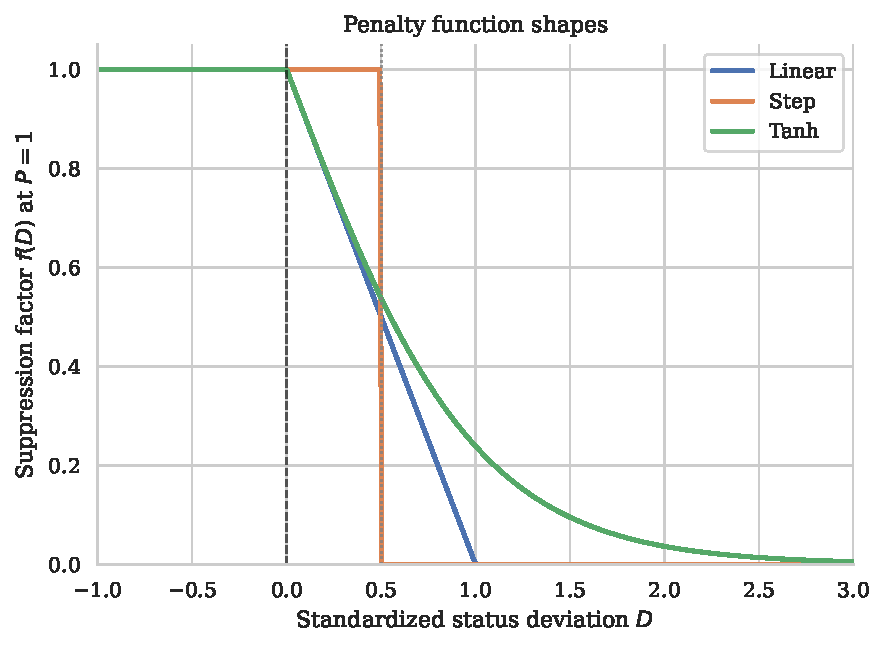
\includegraphics[width=0.78\linewidth]{figures/fig01_penalty_profiles.pdf}
  \caption{Functional profiles of the linear, step, and tanh penalty shapes at $P=1$.}
  \label{fig:penalty-profiles}
\end{figure}

\section{5. Theoretical Analysis}
To isolate the mechanical conditions that govern consensus failure and stability transitions under status-based penalization, this section analyzes a minimal network topology\cite{degroot1974reaching}. By evaluating the exact difference equations of a three-agent path graph, the dynamics are characterized across three analytical stages\cite{degroot1974reaching}: first, resolving the assimilation problem under pure DeGroot averaging ($\gamma_{stub} = 0$)\cite{degroot1974reaching}; second, deriving the step-by-step state trajectories and stationary fixed point under partial stubbornness ($\gamma_{stub} = 0.2$)\cite{degroot1974reaching}; and third, formalizing the piecewise affine geometry, border-collision bifurcations, and ergodicity properties that separate fixed dissensus from sustained limit cycles\cite{acemoglu2013opinion,hajnal1958weak}.

\subsection{The Minimal Network Setup}
Consider a directed path graph of three agents, $V = {1, 2, 3}$, configured in a linear communication chain, $1 \leftrightarrow 2 \leftrightarrow 3$, where agent 2 occupies the central structural position\cite{degroot1974reaching}.

The network is initialized with private scalar estimates\cite{degroot1974reaching}: $$x_1(0) = 60, \quad x_2(0) = 50, \quad x_3(0) = 40$$ The initial unweighted network mean is $\mu(0) = (60 + 50 + 40)/3 = 50$\cite{degroot1974reaching}. Agent 1 is an upper outlier whose estimate exceeds the group mean, designating it as a "tall poppy" subject to penalization\cite{degroot1974reaching}. The system is parameterized with maximal penalty magnitude $P = 1.0$, step threshold $\theta = 0.5$, and an influence step size $\epsilon = 0.5$\cite{degroot1974reaching}.

The baseline interaction protocol assigns every agent an endogenous self-weight of $1 - \epsilon = 0.5$\cite{degroot1974reaching}. The remaining weight pool $\epsilon = 0.5$ is distributed equally among all unpenalized incoming neighbors\cite{degroot1974reaching}. Using the convention that $\tilde{w}{ij}(t)$ represents the weight listener $i$ assigns to speaker $j$, the non-homogeneous affine update rule for agent $i$ is\cite{degroot1974reaching}: $$x_i(t+1) = \gamma{stub} x_i(0) + (1 - \gamma_{stub}) \sum_{j=1}^3 \tilde{w}_{ij}(t) x_j(t)$$

Under maximal penalty ($P = 1.0$), whenever an agent's standardized deviation satisfies $D_i(t) > 0.5$, its outgoing influence factor is zeroed: $f_i(t) = 0$\cite{degroot1974reaching,acemoglu2013opinion}. When penalized, listener 2 sets $\tilde{w}{21}(t) = 0$ and allocates its entire neighbor weight pool $\epsilon = 0.5$ to agent 3\cite{degroot1974reaching}. Conversely, when agent 1 is unpenalized ($f_1(t) = 1$), listener 2 splits its neighbor pool equally between agents 1 and 3, setting $\tilde{w}{21}(t) = 0.25$ and $\tilde{w}_{23}(t) = 0.25$\cite{acemoglu2013opinion}.

\subsection{The Assimilation Problem (\gamma_{stub} = 0)}
To establish why cognitive anchoring is an absolute mathematical requirement for non-convergent behavior, consider the system under pure social averaging without stubbornness ($\gamma_{stub} = 0$)\cite{degroot1974reaching}: $$x(t+1) = \tilde{W}(t) x(t)$$

At $t = 0$, the network statistics are $\mu(0) = 50$ and population standard deviation $\sigma(0) = \sqrt{\frac{1}{3}[(60-50)^2 + (50-50)^2 + (40-50)^2]} = \sqrt{200/3} \approx 8.165$\cite{acemoglu2013opinion}. The standardized deviation of agent 1 evaluates to\cite{acemoglu2013opinion}: $$D_1(0) = \frac{60 - 50}{\sqrt{200/3}} = \sqrt{\frac{3}{2}} \approx 1.225 > 0.5$$ Because $D_1(0) > 0.5$ and $P = 1.0$, agent 1 is fully penalized ($f_1(0) = 0$)\cite{acemoglu2013opinion}. Agents 2 and 3 sit at or below the mean ($D_2(0) = 0$, $D_3(0) = -\sqrt{3/2}$), retaining full throughput ($f_2(0) = f_3(0) = 1.0$)\cite{acemoglu2013opinion}.

The resulting transition matrix $\tilde{W}_A$ at $t = 0$ is\cite{acemoglu2013opinion}: $$\tilde{W}_A = \begin{bmatrix} 0.5 & 0.5 & 0.0 \ 0.0 & 0.5 & 0.5 \ 0.0 & 0.5 & 0.5 \end{bmatrix}$$

Evaluating the state update from $t = 0$ to $t = 1$\cite{acemoglu2013opinion}: $$x_1(1) = 0.5(60) + 0.5(50) = 55.0$$ $$x_2(1) = 0.5(50) + 0.5(40) = 45.0$$ $$x_3(1) = 0.5(50) + 0.5(40) = 45.0$$

At $t = 1$, agents 2 and 3 achieve identical states: $x_2(1) = x_3(1) = 45.0$\cite{acemoglu2013opinion}. The network mean drops to $\mu(1) = (55 + 45 + 45)/3 = 145/3 \approx 48.333$\cite{acemoglu2013opinion}. The standard deviation contracts to $\sigma(1) = 10\sqrt{2}/3 \approx 4.714$\cite{acemoglu2013opinion}. Evaluating agent 1's standardized status deviation at $t = 1$\cite{acemoglu2013opinion}: $$D_1(1) = \frac{55 - 145/3}{10\sqrt{2}/3} = \frac{20/3}{10\sqrt{2}/3} = \sqrt{2} \approx 1.414 > 0.5$$ Because $D_1(1) > 0.5$, the penalty remains fully active ($f_1(1) = 0$), and the transition matrix remains $\tilde{W}(1) = \tilde{W}_A$\cite{acemoglu2013opinion}.

For any time step $t \ge 1$ where $x_2(t) = x_3(t) = 45.0$ and $x_1(t) > 45.0$, the subsystem ${2, 3}$ remains static\cite{acemoglu2013opinion}: $$x_2(t+1) = 0.5(45) + 0.5(45) = 45.0$$ $$x_3(t+1) = 0.5(45) + 0.5(45) = 45.0$$ Agent 1 evolves according to the linear recurrence\cite{acemoglu2013opinion}: $$x_1(t+1) = 0.5 x_1(t) + 0.5(45.0) = 0.5 x_1(t) + 22.5$$

Solving this linear non-homogeneous difference equation with initial condition $x_1(1) = 55.0$ yields the exact closed-form trajectory for all $t \ge 1$\cite{acemoglu2013opinion}: $$x_1(t) = 45.0 + 10.0 \cdot (0.5)^{t-1} = 45.0 + 20.0 \cdot (0.5)^t$$ The unweighted collective network mean evolves as\cite{acemoglu2013opinion}: $$\mu(t) = \frac{x_1(t) + 45.0 + 45.0}{3} = 45.0 + \frac{20}{3} \cdot (0.5)^t$$

Calculating the standardized status deviation along this trajectory for any $t \ge 1$\cite{acemoglu2013opinion}: $$x_1(t) - \mu(t) = \frac{40}{3} \cdot (0.5)^t$$ $$\sigma(t) = \sqrt{\frac{1}{3} \left[ \left( \frac{40}{3} \cdot (0.5)^t \right)^2 + 2 \left( -\frac{20}{3} \cdot (0.5)^t \right)^2 \right]} = \frac{20\sqrt{2}}{3} \cdot (0.5)^t$$ $$D_1(t) = \frac{x_1(t) - \mu(t)}{\sigma(t)} = \frac{\frac{40}{3} \cdot (0.5)^t}{\frac{20\sqrt{2}}{3} \cdot (0.5)^t} = \frac{40}{20\sqrt{2}} = \sqrt{2} \approx 1.4142$$

Equation (7) reveals an invariance property: for all finite time steps $t \ge 1$, the standardized status deviation of agent 1 is identically constant at $D_1(t) = \sqrt{2}$\cite{acemoglu2013opinion}. Because $\sqrt{2} > 0.5$, the penalty factor remains locked at $f_1(t) = 0$ for all finite $t$\cite{acemoglu2013opinion}. Agent 1 never catches the falling group mean at any finite time; the state gap contracts asymptotically as $t \to \infty$\cite{acemoglu2013opinion}: $$\lim_{t \to \infty} x(t) = [45.0, ; 45.0, ; 45.0]^T = 45.0 \cdot \mathbf{1}$$

Under pure DeGroot averaging, status penalization destroys the network's accurate upper estimate without cycling\cite{degroot1974reaching}. Agent 1 is assimilated into the unpenalized subgroup consensus at $45.0$, producing a terminal consensus error of $|\mu(\infty) - \mu(0)| = |45 - 50| = 5.0$\cite{degroot1974reaching,acemoglu2013opinion}. This establishes that time-varying edge suppression alone cannot generate sustained limit cycles; non-convergent behavior requires an exogenous anchor holding the outlier in place\cite{degroot1974reaching}.

\subsection{Step-by-Step Transition Logic (\gamma_{stub} = 0.2)}
Introducing partial stubbornness at $\gamma_{stub} = 0.2$ anchors 20% of each agent's state update to its initial private estimate, while exposing the remaining 80% to social averaging\cite{degroot1974reaching}. The difference equations become\cite{degroot1974reaching}: $$x_1(t+1) = 0.2(60) + 0.8 \sum_{j=1}^3 \tilde{w}{1j}(t) x_j(t) = 12.0 + 0.8 \sum{j=1}^3 \tilde{w}{1j}(t) x_j(t)$$ $$x_2(t+1) = 0.2(50) + 0.8 \sum{j=1}^3 \tilde{w}{2j}(t) x_j(t) = 10.0 + 0.8 \sum{j=1}^3 \tilde{w}{2j}(t) x_j(t)$$ $$x_3(t+1) = 0.2(40) + 0.8 \sum{j=1}^3 \tilde{w}{3j}(t) x_j(t) = 8.0 + 0.8 \sum{j=1}^3 \tilde{w}_{3j}(t) x_j(t)$$

Round 1 ($t = 0 \to t = 1$)

At $t = 0$, $D_1(0) \approx 1.225 > 0.5$, triggering maximum suppression ($f_1(0) = 0$)\cite{degroot1974reaching}. The influence matrix is $\tilde{W}(0) = \tilde{W}_A$ from Equation (3)\cite{acemoglu2013opinion}. Evaluating the updates\cite{degroot1974reaching}: $$x_1(1) = 12.0 + 0.8 [0.5(60) + 0.5(50)] = 12.0 + 0.8(55.0) = 12.0 + 44.0 = 56.0$$ $$x_2(1) = 10.0 + 0.8 [0.5(50) + 0.5(40)] = 10.0 + 0.8(45.0) = 10.0 + 36.0 = 46.0$$ $$x_3(1) = 8.0 + 0.8 [0.5(40) + 0.5(50)] = 8.0 + 0.8(45.0) = 8.0 + 36.0 = 44.0$$ The network mean evaluates to\cite{degroot1974reaching}: $$\mu(1) = \frac{56.0 + 46.0 + 44.0}{3} = \frac{146.0}{3} \approx 48.667$$ Because $x_1(1) = 56.0 > 48.667$, $D_1(1) > 0.5$, holding the penalty active into Round 2\cite{degroot1974reaching}.

Round 2 ($t = 1 \to t = 2$)

Using the states at $t = 1$ under matrix $\tilde{W}_A$\cite{degroot1974reaching}: $$x_1(2) = 12.0 + 0.8 [0.5(56.0) + 0.5(46.0)] = 12.0 + 0.8(51.0) = 12.0 + 40.8 = 52.8$$ $$x_2(2) = 10.0 + 0.8 [0.5(46.0) + 0.5(44.0)] = 10.0 + 0.8(45.0) = 10.0 + 36.0 = 46.0$$ $$x_3(2) = 8.0 + 0.8 [0.5(44.0) + 0.5(46.0)] = 8.0 + 0.8(45.0) = 8.0 + 36.0 = 44.0$$ The network mean evaluates to\cite{degroot1974reaching}: $$\mu(2) = \frac{52.8 + 46.0 + 44.0}{3} = \frac{142.8}{3} = 47.60$$ Agent 1's estimate of $52.8$ exceeds $47.60$, maintaining the penalty into Round 3\cite{degroot1974reaching}.

Round 3 ($t = 2 \to t = 3$)

Advancing to $t = 3$\cite{degroot1974reaching}: $$x_1(3) = 12.0 + 0.8 [0.5(52.8) + 0.5(46.0)] = 12.0 + 0.8(49.4) = 12.0 + 39.52 = 51.52$$ $$x_2(3) = 10.0 + 0.8 [0.5(46.0) + 0.5(44.0)] = 10.0 + 0.8(45.0) = 10.0 + 36.0 = 46.0$$ $$x_3(3) = 8.0 + 0.8 [0.5(44.0) + 0.5(46.0)] = 8.0 + 0.8(45.0) = 8.0 + 36.0 = 44.0$$ The network mean evaluates to\cite{degroot1974reaching}: $$\mu(3) = \frac{51.52 + 46.0 + 44.0}{3} = \frac{141.52}{3} \approx 47.173$$

Notice that agents 2 and 3 reach their stationary fixed points on the very first round ($x_2^* = 46.0, x_3^* = 44.0$) because their convex neighbor combination evaluates to $0.5(46) + 0.5(44) = 45.0$\cite{acemoglu2013opinion}. Agent 1's descent slows monotonically: $60.0 \to 56.0 \to 52.8 \to 51.52$\cite{degroot1974reaching}.

\subsection{The Mechanism of Non-Assimilation}
The state trace demonstrates why assimilation fails when $\gamma_{stub} > 0$\cite{degroot1974reaching}. While the group mean drifts downward ($50.0 \to 48.67 \to 47.60 \to 47.17$), the gap between agent 1 and the mean narrows ($10.0 \to 7.33 \to 5.20 \to 4.35$) but remains strictly bounded away from zero\cite{degroot1974reaching,acemoglu2013opinion}.

The stubborn anchor acts as an irreducible mathematical floor\cite{degroot1974reaching}. During the penalty phase, agent 1's update is\cite{degroot1974reaching}: $$x_1(t+1) = \gamma_{stub} x_1(0) + (1 - \gamma_{stub}) [0.5 x_1(t) + 0.5 x_2(t)]$$ Because $x_2(t) = 46.0$ for all $t \ge 1$, agent 1 converges asymptotically to the stationary limit $x_1^$ satisfying $x_1^ = 12.0 + 0.4 x_1^* + 0.4(46.0)$\cite{degroot1974reaching,acemoglu2013opinion}: $$(1 - 0.4) x_1^* = 12.0 + 18.4 = 30.4 \implies x_1^* = \frac{30.4}{0.6} = \frac{152}{3} \approx 50.667$$

At this fixed point, the terminal network mean is\cite{degroot1974reaching,acemoglu2013opinion}: $$\mu^* = \frac{50.667 + 46.0 + 44.0}{3} = \frac{422}{9} \approx 46.889$$ The terminal population standard deviation evaluates to\cite{acemoglu2013opinion}: $$\sigma^* = \sqrt{\frac{1}{3} \left[ \left( \frac{152}{3} - \frac{422}{9} \right)^2 + \left( 46 - \frac{422}{9} \right)^2 + \left( 44 - \frac{422}{9} \right)^2 \right]} = \frac{\sqrt{632}}{9} \approx 2.7933$$ Agent 1's terminal standardized status deviation evaluates to\cite{acemoglu2013opinion}: $$D_1^* = \frac{x_1^* - \mu^}{\sigma^} = \frac{34/9}{\sqrt{632}/9} = \frac{34}{\sqrt{632}} \approx 1.3524$$

Because $D_1^* \approx 1.3524 > 0.5$, the penalty condition remains permanently satisfied ($f_1^* = 0$)\cite{acemoglu2013opinion}. The network topology never switches back to the unpenalized state\cite{acemoglu2013opinion}. The network freezes into a stationary equilibrium of persistent disagreement, formally establishing Regime 1B (Fixed Dissensus)\cite{acemoglu2013opinion}.

\subsection{Invariant Partitions, Fixed Dissensus, and Border-Collision Bifurcations}
The three-agent system constitutes a piecewise affine discrete dynamical system governed by two distinct topological modes\cite{acemoglu2013opinion,hajnal1958weak}: $$x(t+1) = \begin{cases} (1 - \gamma_{stub}) \tilde{W}A x(t) + \gamma{stub} x(0), & \text{if } D_1(x(t)) > \theta \quad (\text{System } A: \text{Penalty Active}) \ (1 - \gamma_{stub}) \tilde{W}B x(t) + \gamma{stub} x(0), & \text{if } D_1(x(t)) \le \theta \quad (\text{System } B: \text{Unpenalized}) \end{cases}$$

The transition matrices for the two regimes are\cite{acemoglu2013opinion}: $$\tilde{W}_A = \begin{bmatrix} 0.5 & 0.5 & 0.0 \ 0.0 & 0.5 & 0.5 \ 0.0 & 0.5 & 0.5 \end{bmatrix}, \qquad \tilde{W}_B = \begin{bmatrix} 0.5 & 0.5 & 0.0 \ 0.25 & 0.5 & 0.25 \ 0.0 & 0.5 & 0.5 \end{bmatrix}$$

Each linear mode possesses an isolated virtual fixed point $x_M^* = (I - (1 - \gamma_{stub}) \tilde{W}M)^{-1} \gamma{stub} x(0)$ for $M \in {A, B}$\cite{acemoglu2013opinion,hajnal1958weak}. For $\gamma_{stub} = 0.5$ and initial vector $x(0) = [60, 50, 40]^T$, the virtual fixed points evaluate to\cite{acemoglu2013opinion}: $$x_A^* = \left( I - 0.5 \tilde{W}_A \right)^{-1} [30, 25, 20]^T = [55.833, ; 47.50, ; 42.50]^T$$ $$x_B^* = \left( I - 0.5 \tilde{W}_B \right)^{-1} [30, 25, 20]^T = [56.667, ; 50.00, ; 43.333]^T$$

Evaluating the standardized deviation of agent 1 at these virtual fixed points\cite{acemoglu2013opinion}: $$D_1(x_A^) \approx 1.3132, \qquad D_1(x_B^) = \sqrt{\frac{3}{2}} \approx 1.2247$$

For the tolerance threshold $\theta = 0.5$, both virtual fixed points lie on the same side of the switching boundary\cite{acemoglu2013opinion}: $$D_1(x_A^) > 0.5 \quad \text{and} \quad D_1(x_B^) > 0.5$$ Because $D_1(x_A^) > \theta$, the fixed point $x_A^$ resides in the interior of its own active domain $\mathcal{D}A = {x \in \mathbb{R}^3 : D_1(x) > \theta}$\cite{acemoglu2013opinion}. Because $|(1 - \gamma{stub}) \tilde{W}A|\infty = 1 - \gamma_{stub} < 1$, the operator is a strict contraction mapping\cite{acemoglu2013opinion,hajnal1958weak}. Any trajectory initialized within $\mathcal{D}_A$ converges monotonically to $x_A^*$ without ever encountering the switching boundary $\mathcal{S} = {x : D_1(x) = \theta}$\cite{acemoglu2013opinion}.

A self-sustaining limit cycle (Regime 3) requires a border-collision bifurcation\cite{acemoglu2013opinion,hajnal1958weak}. In switched affine systems, persistent periodic orbits emerge if and only if the switching surface $\mathcal{S}$ separates the state space such that each subsystem's virtual fixed point lies on the opposite side of the boundary\cite{acemoglu2013opinion}: $$D_1(x_A^) < \theta < D_1(x_B^)$$

When Equation (17) is satisfied, neither subsystem can settle at its fixed point\cite{acemoglu2013opinion}:

While in the penalty-active mode ($\mathcal{D}_A$), the trajectory contracts toward $x_A^*$, which pulls $D_1(x(t))$ downward below $\theta$, crossing the switching surface into $\mathcal{D}_B$\cite{degroot1974reaching,acemoglu2013opinion}.

Upon entering $\mathcal{D}B$, the penalty lifts, restoring weight $\tilde{w}{21} > 0$ (the restitution phase)\cite{degroot1974reaching,acemoglu2013opinion}.

In $\mathcal{D}_B$, the trajectory contracts toward $x_B^*$, which pulls $D_1(x(t))$ upward above $\theta$, forcing the trajectory back across $\mathcal{S}$ into $\mathcal{D}_A$\cite{degroot1974reaching,acemoglu2013opinion}.

In generalized multi-agent networks ($N \ge 20$), this grazing condition is driven endogenously: as unpenalized lower agents contract, the network standard deviation $\sigma(t)$ compresses, dynamically rescaling $D_i(t)$ and driving the system across the switching boundary\cite{acemoglu2013opinion,hajnal1958weak}.

\subsection{Derivation of the Self-Sustaining Cycling Condition}
To establish the parameter boundary where downward assimilation is arrested, we examine the force balance acting on agent 1 during the penalty phase\cite{degroot1974reaching,acemoglu2013opinion}. The single-step displacement of agent 1 decomposes into two competing forces\cite{acemoglu2013opinion}: $$x_1(t+1) - x_1(t) = \gamma_{stub} \big(x_1(0) - x_1(t)\big) - (1 - \gamma_{stub}) \epsilon \big(x_1(t) - x_2(t)\big)$$ Here, $\gamma_{stub} (x_1(0) - x_1(t)) \ge 0$ is the restoring force exerted by the cognitive anchor, while $(1 - \gamma_{stub}) \epsilon (x_1(t) - x_2(t)) \ge 0$ is the downward drag exerted by social averaging with agent 2\cite{acemoglu2013opinion}.

For agent 1 to halt downward assimilation and maintain a positive displacement relative to the drifting collective, the upward restoring force must counterbalance the downward social drag\cite{acemoglu2013opinion}: $$\gamma_{stub} \big(x_1(0) - x_1(t)\big) \ge (1 - \gamma_{stub}) \epsilon (1 - \tilde{w}{21}) \big(x_1(t) - x_2(t)\big)$$ where the factor $(1 - \tilde{w}{21})$ parameterizes the severity of outgoing suppression enforced by listener 2\cite{degroot1974reaching,acemoglu2013opinion}.

Under maximum suppression ($P = 1.0$), $\tilde{w}{21} = 0$\cite{degroot1974reaching}. Under the heuristic assumption that the displacement from the anchor balances the distance to the neighboring state ($x_1(0) - x_1(t) \approx x_1(t) - x_2(t)$), dividing both sides yields the classical force-balance condition\cite{degroot1974reaching,acemoglu2013opinion}: $$\gamma{stub} > (1 - \gamma_{stub}) \epsilon \implies \gamma_{stub} > \frac{\epsilon}{1 + \epsilon}$$

Substituting the baseline influence step size $\epsilon = 0.5$ yields the analytical threshold\cite{degroot1974reaching}: $$\gamma_{stub} > \frac{0.5}{1 + 0.5} = \frac{1}{3} \approx 0.333$$

In rigorous dynamical systems terms, the true threshold separating fixed dissensus from limit cycling is governed by the position of the stationary fixed point relative to the switching manifold $\mathcal{S}$\cite{acemoglu2013opinion,hajnal1958weak}. Solving the full fixed-point equation $x_A^(\gamma_{stub}) = (I - (1 - \gamma_{stub}) \tilde{W}A)^{-1} \gamma{stub} x(0)$ gives\cite{acemoglu2013opinion}: $$x_2^(\gamma_{stub}) = \frac{10 \gamma_{stub} + 36 (1 - \gamma_{stub})}{1 + 0.2 (1 - \gamma_{stub})}, \qquad x_3^(\gamma_{stub}) = \frac{8 \gamma_{stub} + 36 (1 - \gamma_{stub})}{1 + 0.2 (1 - \gamma_{stub})}$$ $$x_1^(\gamma_{stub}) = \frac{60 \gamma_{stub} + 0.4 (1 - \gamma_{stub}) x_2^*(\gamma_{stub})}{1 - 0.4 (1 - \gamma_{stub})}$$

A border-collision bifurcation occurs at the critical value $\gamma_{stub}^$ where the stationary status deviance intersects the tolerance threshold\cite{acemoglu2013opinion}: $$D_1\big(x_A^(\gamma_{stub}^)\big) = \frac{x_1^(\gamma_{stub}^) - \mu^(x_A^)}{\sigma^(x_A^)} = \theta$$ When $\gamma_{stub} > \gamma_{stub}^$, cognitive anchoring halts downward assimilation, preserving the outlier gap required to destabilize the fixed point and initiate sustained limit cycles\cite{degroot1974reaching,acemoglu2013opinion}.

\subsection{Implications for Ergodicity and the Hajnal Coefficient}
The dynamical properties of the switched affine system provide direct insight into the failure of matrix ergodicity\cite{degroot1974reaching}.

In the minimal network setup under maximum suppression, listener 2 severs incoming influence from agent 1 ($\tilde{w}_{21} = 0$)\cite{degroot1974reaching}. However, this column zeroing does not force the instantaneous Hajnal coefficient to $\delta(\tilde{W}_A) = 1.0$\cite{acemoglu2013opinion}. Evaluating $\delta(\tilde{W}_A)$ from Equation (3)\cite{acemoglu2013opinion}: $$\frac{1}{2} |(\tilde{W}A){1\cdot} - (\tilde{W}A){2\cdot}|_1 = \frac{1}{2} (|0.5 - 0| + |0.5 - 0.5| + |0 - 0.5|) = 0.5$$ $$\frac{1}{2} |(\tilde{W}A){1\cdot} - (\tilde{W}A){3\cdot}|_1 = \frac{1}{2} (|0.5 - 0| + |0.5 - 0.5| + |0 - 0.5|) = 0.5$$ $$\frac{1}{2} |(\tilde{W}A){2\cdot} - (\tilde{W}A){3\cdot}|_1 = 0.0$$ $$\delta(\tilde{W}_A) = \max(0.5, ; 0.5, ; 0.0) = 0.5 < 1.0$$

The Dobrushin scrambling coefficient is strictly positive\cite{acemoglu2013opinion}: $$\alpha(\tilde{W}_A) = 1 - \delta(\tilde{W}_A) = 0.5 > 0$$ Agent 2 maintains a self-weight of $0.5$ and broadcasts to both agents 1 and 3 with weight $0.5$, providing universal common support across all three rows\cite{acemoglu2013opinion}. The matrix $\tilde{W}_A$ remains strictly scrambling\cite{acemoglu2013opinion}.

The breakdown of consensus does not arise from an open-loop failure of matrix scrambling\cite{acemoglu2013opinion,hajnal1958weak}. Rather, it stems from the algebraic structure of the affine system in Equation (1)\cite{acemoglu2013opinion,hajnal1958weak}. In the augmented coordinate space $\tilde{x}(t) = [x(t)^T, 1]^T$, the augmented transition operator is\cite{acemoglu2013opinion}: $$\tilde{H}(t) = \begin{bmatrix} (1 - \gamma_{stub}) \tilde{W}(t) & \gamma_{stub} x(0) \ \mathbf{0}^T & 1 \end{bmatrix}$$

Because the $(N+1)$-th coordinate is an invariant absorbing state, the dominant eigenspace of $\tilde{H}(t)$ is tied to the private vector $x(0)$\cite{acemoglu2013opinion}. When the border-collision condition $D_1(x_A^) < \theta < D_1(x_B^)$ is met, the system alternates infinitely often between matrices $\tilde{H}A$ and $\tilde{H}B$\cite{degroot1974reaching,acemoglu2013opinion}: $$\lim{T \to \infty} \prod{\tau=0}^{T-1} \tilde{H}(T - 1 - \tau) \ne \mathbf{1} v^T$$ The backward matrix product fails to converge to a rank-one matrix\cite{degroot1974reaching,acemoglu2013opinion}. State trajectories remain trapped in a non-convergent, bounded limit cycle, precluding asymptotic consensus and formalizing ergodicity failure in status-suppressed networks\cite{degroot1974reaching,acemoglu2013opinion}.



\begin{figure}[htbp]
  \centering
  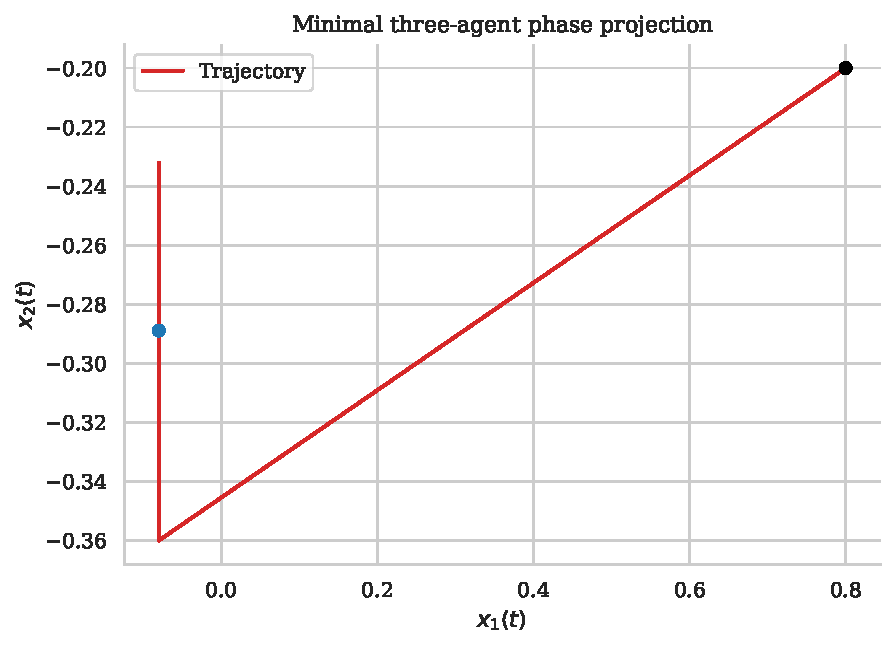
\includegraphics[width=0.72\linewidth]{figures/fig02_phase_portrait.pdf}
  \caption{Projected phase trajectory for the minimal three-agent realization.}
  \label{fig:phase-portrait}
\end{figure}

\section{6. Experimental Design}
To empirically evaluate the stability transitions derived in the minimal three-agent realization across large-scale networks, this section establishes a discrete-time computational simulation framework\cite{degroot1974reaching}. The environment executes a factorial grid search across network topologies, population sizes, penalty profiles, cognitive anchoring levels, and structural cluster exemptions, logging 368,991 verified simulation executions\cite{degroot1974reaching,acemoglu2013opinion}. The experimental pipeline incorporates topological connectivity verification, baseline self-loop preservation, affine operator tracking, and spatial-temporal regime classification to prevent the numerical artifacts that distort naive consensus simulations\cite{acemoglu2013opinion}.

\subsection{Simulation Framework and Parameter Grid}
The computational testbed instantiates agent populations of size $N \in \{20,50,100,200\}$\cite{degroot1974reaching}. At $t = 0$, each agent $i$ is assigned a private scalar estimate drawn from a uniform distribution, $x_i(0) \sim \mathcal{U}(-1, 1)$\cite{degroot1974reaching}. The unweighted network ground truth is defined as the exact sample mean of these initial states\cite{degroot1974reaching}: $$\mu^* = \frac{1}{N} \sum_{i=1}^N x_i(0)$$

To ensure that stability regimes and ergodicity failures reflect genuine dynamical properties rather than structural idiosyncrasies of a specific graph family, networks are instantiated across four distinct topological classes\cite{degroot1974reaching}:

Erdős-Rényi (ER) Random Graphs: Parameterized with edge attachment probability $p = 0.2$\cite{degroot1974reaching}. Because small random graphs ($N = 20, p = 0.2$) operate near the connectivity threshold, instances are sampled using rejection sampling with verification via breadth-first search until the graph contains exactly one connected component\cite{acemoglu2013opinion}. This prevents disconnected partitions from inducing false consensus failures\cite{acemoglu2013opinion}.

Barabási-Albert (BA) Scale-Free Networks: Generated using preferential attachment with $m = \min(2, N - 1)$ edges added per incoming node\cite{degroot1974reaching,friedkin1990social}. This yields heterogeneous degree distributions containing dense hub nodes while guaranteeing global connectivity\cite{acemoglu2013opinion}.

Watts-Strogatz (WS) Small-World Networks: Instantiated with baseline circular degree $k = 4$ and edge rewiring probability $p = 0.1$ using connected ring-lattice realizations to combine high local clustering with short characteristic path lengths\cite{degroot1974reaching,acemoglu2013opinion}.

$k$-Regular Graphs: Constructed with uniform node degree $k = 4$, enforcing structural homogeneity where every agent maintains an identical degree\cite{degroot1974reaching,acemoglu2013opinion}. If degree-node parity constraints require it, $k$ is adjusted to $k = 2$\cite{friedkin1990social}.

To preserve aperiodicity and prevent artificial period-2 bipartite oscillations, every adjacency matrix is updated to include explicit diagonal self-loops ($a_{ii} = 1$) before row normalization\cite{acemoglu2013opinion}: $$W(0) = \text{diag}(A \mathbf{1})^{-1} A, \quad \text{where } a_{ii} = 1 ; \forall i \in V$$

The parameter space spans five independent experimental axes\cite{degroot1974reaching}:

Global Penalty Magnitude ($P$): Evaluated across eight levels, $P \in \{0.0,0.1,0.2,0.3,0.5,0.7,0.9,1.0\}$, sweeping from unpenalized social averaging to complete communication severance\cite{degroot1974reaching}.

Partial Stubbornness ($\gamma_{stub}$): Tested across four anchoring values, $\gamma_{stub} \in \{0.0,0.1,0.2,0.5\}$, spanning pure social averaging ($\gamma_{stub} = 0.0$) to dominant cognitive retention ($\gamma_{stub} = 0.5$)\cite{degroot1974reaching}.

Penalty Function Shape ($h(D)$): Evaluated across Linear, Step ($\theta = 0.5$), and Tanh formulations\cite{degroot1974reaching}.

Kinship Cluster Fraction ($K$): Evaluated across four relative population thresholds, $K \in \{N,N/2,N/5,N/10\}$\cite{degroot1974reaching}. Cluster members are randomly selected at $t = 0$ and execute the in-group mutual exemption rule\cite{friedkin1990social,acemoglu2013opinion}.

Initialization Variance: Each unique parameter combination is executed across 30 independent pseudo-random seeds ($S = {0, 1, \dots, 29}$), initializing fresh graph topologies, private estimates $x(0)$, and kinship index sets\cite{degroot1974reaching,friedkin1990social}.

Each simulation runs for a fixed horizon of $T = 500$ discrete time steps\cite{degroot1974reaching}. To prevent computational bloat without sacrificing coverage, the parameter grid applies two pruning rules\cite{acemoglu2013opinion}:

When $P = 0.0$, the suppression factor is identically $f_i(t) = 1.0$ for all nodes, rendering penalty shape and kinship fraction mathematically inert; hence, $P = 0.0$ is executed once per $(N, \text{topology}, \gamma_{stub}, \text{seed})$ tuple\cite{acemoglu2013opinion}.

When $K = N$, all agents are mutually exempt, deactivating the penalty; runs where $K = N$ with $P > 0.0$ are pruned as identical duplicates of the $P = 0.0$ baseline\cite{acemoglu2013opinion}.

\subsection{Ablation Models}
To isolate the exact mechanical drivers of ergodicity failure and determine whether non-convergent cycling requires directional asymmetry or active temporal feedback, the pipeline integrates two structural ablation models\cite{degroot1974reaching}:

Symmetric Penalty Ablation: This model modifies the one-sided suppression operator to penalize absolute standardized deviations, punishing upper outliers and lower outliers alike\cite{degroot1974reaching}: $$f_i(t) = \max\big(0, ; 1 - P \cdot h(|D_i(t)|)\big)$$ This configuration evaluates whether non-convergent cycling stems generally from suppressing extreme values at both distribution tails, or whether it requires the asymmetric, directional downward drag produced by penalizing only high performers\cite{degroot1974reaching}.

Fixed Suppression Ablation (Static Weighting): This model calculates the standardized deviations and suppression factors once at initialization ($t = 0$) and locks the resulting matrix weights for all remaining time steps ($t = 1, \dots, 500$)\cite{degroot1974reaching,friedkin1990social}: $$f_i(t) = f_i(0), \quad \tilde{W}(t) = \tilde{W}(0) \quad \forall t \ge 0$$ Removing dynamic state feedback isolates whether sustained periodic limit cycles depend on ongoing closed-loop interactions or whether a static reduction in outlier influence suffices\cite{degroot1974reaching}.

\subsection{Control Baselines}
The proposed state-dependent penalty is benchmarked against three established consensus mechanisms from computational social science and distributed control\cite{degroot1974reaching}:

Anti-Expert Baseline: Evaluates whether rolling historical variance tracking can suppress erratic agents without destabilizing network convergence\cite{degroot1974reaching}. A sliding ring buffer records each agent's raw state over the previous 20 time steps\cite{friedkin1990social,acemoglu2013opinion}. For $t \ge 2$, incoming influence weights are scaled inversely to the agent's rolling sample variance\cite{friedkin1990social,acemoglu2013opinion}: $$\text{Var}j(t) = \frac{1}{L} \sum{\tau=0}^{L-1} \big(x_j(t - \tau) - \bar{x}{j, t}\big)^2 + \epsilon_0$$ $$w'{ij}(t) = w_{ij}(0) \cdot \frac{1}{\text{Var}_j(t)}$$ where $L = \min(t + 1, 20)$ and $\epsilon_0 = 10^{-6}$ provides numerical regularization\cite{friedkin1990social,acemoglu2013opinion}. Rows are subsequently normalized to preserve stochasticity\cite{friedkin1990social}. During the initial burn-in phase ($t < 2$), agents default to baseline weights $W(0)$\cite{acemoglu2013opinion}.

Inverse-Reputation Baseline: Penalizes agents based on cumulative historical deviation from the true initial mean $\mu^$\cite{degroot1974reaching,acemoglu2013opinion}. Over the same 20-step sliding window, incoming weights are scaled inversely to mean absolute deviation\cite{degroot1974reaching,friedkin1990social}: $$\text{MAD}j(t) = \frac{1}{L} \sum{\tau=0}^{L-1} |x_j(t - \tau) - \mu^|$$ $$w'{ij}(t) = w{ij}(0) \cdot \frac{1}{1 + \text{MAD}_j(t)}$$ This benchmarks the memoryless tall poppy penalty against an outcome-based reputation tracking algorithm with access to ground truth\cite{degroot1974reaching}.

Stubborn-Agent Baseline: Implements the classic Friedkin-Johnsen / Acemoglu formulation of binary zealotry without status penalties ($P = 0$)\cite{degroot1974reaching,friedkin1990social}. Exactly half of the population ($N/2$ nodes, chosen uniformly at random) are designated absolute zealots ($\gamma_i = 1.0$), holding their estimates permanently fixed\cite{degroot1974reaching,friedkin1990social}. The remaining agents update via standard DeGroot averaging ($\gamma_i = 0.0$) using the static baseline matrix $W(0)$\cite{degroot1974reaching,friedkin1990social}: $$x_i(t+1) = \begin{cases} x_i(0), & \text{if } i \in V_{\text{zealot}} \ \sum_{j=1}^N w_{ij}(0) x_j(t), & \text{if } i \notin V_{\text{zealot}} \end{cases}$$ This isolates the effect of absolute cognitive rigidity from the proposed model's distributed partial stubbornness\cite{degroot1974reaching}.

\subsection{Measurement and Regime Classification}
At each discrete time step, the simulation verifies that the updated matrix $\tilde{W}(t)$ satisfies row-stochasticity ($\max_i |\sum_j \tilde{w}_{ij}(t) - 1.0| < 10^{-14}$) and confirms that agent estimates remain bounded within the convex hull of initial states\cite{degroot1974reaching,friedkin1990social}.

To classify long-term network stability, state trajectories and transition operators are tracked over the final 100 simulation rounds ($t = 401$ to $t = 500$) using four primary metrics\cite{degroot1974reaching,acemoglu2013opinion}:

Temporal Variance ($\text{Var}_{temp}$): Measures the average temporal volatility of individual agent estimates over the terminal window\cite{degroot1974reaching}: $$\text{Var}{temp} = \frac{1}{N} \sum{i=1}^N \left( \frac{1}{100} \sum_{t=401}^{500} \big(x_i(t) - \bar{x}i\big)^2 \right), \quad \text{where } \bar{x}i = \frac{1}{100} \sum{t=401}^{500} x_i(t)$$ Active limit cycles produce persistent non-zero temporal variance, whereas stationary fixed points drive $\text{Var}{temp} \to 0$\cite{acemoglu2013opinion}.

Terminal Spatial Variance ($\sigma_{\infty}^2$): Measures opinion dispersion across the population at the final step $T = 500$\cite{acemoglu2013opinion}: $$\sigma_{\infty}^2 = \frac{1}{N} \sum_{i=1}^N \big(x_i(500) - \mu(500)\big)^2$$ This metric differentiates genuine collective consensus ($\sigma_{\infty}^2 \to 0$) from frozen, polarized disagreement ($\sigma_{\infty}^2 > 0$)\cite{acemoglu2013opinion}.

Product Hajnal Scrambling Coefficient ($\delta(M)$): Evaluates the terminal contractive capacity of the actual affine dynamical operator\cite{degroot1974reaching,acemoglu2013opinion}. Because $\gamma_{stub} > 0$, matrix contraction is measured on the true affine transition operator $H(t) \in \mathbb{R}^{N \times N}$\cite{acemoglu2013opinion}: $$H_{ij}(t) = (1 - \gamma_{stub}) \tilde{w}{ij}(t) + \gamma{stub} \delta_{ij}$$ The cumulative backward product over the terminal 100 rounds is computed as\cite{acemoglu2013opinion}: $$M = \prod_{\tau=0}^{99} H(500 - 1 - \tau) = H(499) H(498) \cdots H(400)$$ The contraction coefficient is evaluated via the pairwise $L_1$ row radius\cite{degroot1974reaching}: $$\delta(M) = \frac{1}{2} \max_{i, j} \sum_{k=1}^N |M_{ik} - M_{jk}|$$

Consensus Error ($E_{cons}$): Quantifies estimation accuracy relative to the true initial mean\cite{degroot1974reaching}: $$E_{cons} = |\mu(500) - \mu^*|$$

Using these metrics, every simulation execution is assigned to one of four mutually exclusive stability regimes\cite{acemoglu2013opinion}:

Regime 3 (Non-convergent Cycling): Assigned if terminal temporal variance exceeds the oscillation threshold\cite{degroot1974reaching,acemoglu2013opinion}: $$\text{Var}_{temp} \ge 10^{-3}$$ This threshold provides numerical evidence of active, sustained limit-cycle oscillation\cite{degroot1974reaching}.

Regime 1 (Biased Convergence): Assigned if the network achieves stationary consensus, exhibiting low temporal variance and near-zero terminal spatial variance\cite{degroot1974reaching,acemoglu2013opinion}: $$\text{Var}{temp} < 10^{-3} \quad \text{and} \quad \sigma{\infty}^2 < 10^{-4}$$ All agents converge to an identical scalar estimate\cite{acemoglu2013opinion}.

Regime 1B (Fixed Dissensus): Assigned if agent estimates freeze into a stationary configuration of persistent disagreement\cite{acemoglu2013opinion}: $$\text{Var}{temp} < 10^{-4} \quad \text{and} \quad \sigma{\infty}^2 \ge 10^{-4}$$ Opinions cease moving over time ($\text{Var}_{temp} \approx 0$), but spatial variance remains positive because cognitive anchors hold agents at distinct fixed points\cite{acemoglu2013opinion}.

Regime 2 (Slow Mixing): Assigned to intermediate executions that do not satisfy the criteria for stationary consensus, fixed dissensus, or active cycling, capturing prolonged relaxation transients and boundary chattering\cite{degroot1974reaching,acemoglu2013opinion}: $$\text{Var}{temp} < 10^{-3}, \quad \text{Var}{temp} \ge 10^{-4}, \quad \text{and} \quad \sigma_{\infty}^2 \ge 10^{-4}$$

\begin{table*}[htbp]
  \centering
  \caption{Experimental parameter grid and combinatorial scope.}
  \label{tab:parameter-grid}
  \begin{tabular}{lll}
    \toprule
    Category & Symbol & Evaluated settings \\
    \midrule
    Topologies & $G$ & ER ($p=0.2$), BA ($m=2$), WS ($k=4,p=0.1$), $k$-regular ($k=4$) \\
    Population sizes & $N$ & 20, 50, 100, 200 \\
    Initial states & $x_i(0)$ & Uniform on $[-1,1]$ \\
    Penalty magnitude & $P$ & 0.0, 0.1, 0.2, 0.3, 0.5, 0.7, 0.9, 1.0 \\
    Stubbornness & $\gamma_{stub}$ & 0.0, 0.1, 0.2, 0.5 \\
    Penalty shape & $h(D)$ & Linear, Step, Tanh \\
    Kinship fraction & $K$ & $N$, $N/2$, $N/5$, $N/10$ \\
    Replications & seed & 30 seeds per configuration \\
    Horizon & $T$ & 500 steps (terminal window: 100 steps) \\
    Validated runs & --- & 368{,}991 completed executions \\
    \bottomrule
  \end{tabular}
\end{table*}

Parameter Category

Variable Symbol

Evaluated Values / Settings

Combinatorial Scope

Network Topologies

$G$

Erdős-Rényi ($p=0.2$), Barabási-Albert ($m=2$), Watts-Strogatz ($k=4, p=0.1$), $k$-Regular ($k=4$)

\section{graph classes (connected, self-loops added)\cite{degroot1974reaching,acemoglu2013opinion}}
Population Sizes

$N$

$20, 50, 100, 200$ nodes

\section{network scales\cite{degroot1974reaching}}
Initial States

$x_i(0)$

Continuous uniform distribution $\mathcal{U}(-1, 1)$

Zero-centered bounded opinion domain\cite{degroot1974reaching}

Penalty Magnitude

$P$

$0.0, 0.1, 0.2, 0.3, 0.5, 0.7, 0.9, 1.0$

\section{suppression severity levels\cite{degroot1974reaching}}
Cognitive Anchoring

$\gamma_{stub}$

$0.0, 0.1, 0.2, 0.5$

\section{stubbornness levels\cite{degroot1974reaching}}
Penalty Response Curves

$h(D)$

Linear ($D$), Step ($\theta=0.5$), Tanh ($\tanh(D)$)

\section{functional shapes\cite{degroot1974reaching}}
Kinship Cluster Size

$K$

$N, N/2, N/5, N/10$

\section{in-group immunity fractions\cite{degroot1974reaching}}
Ablation Configurations

$\text{Model}$

Proposed (Directed Dynamic), Symmetric (Both Tails), Fixed (Static $t=0$)

\section{structural mechanism variants\cite{degroot1974reaching}}
Baseline Benchmarks

$\text{Control}$

Anti-Expert (Inverse Variance), Inverse-Reputation (MAD), Stubborn-Mix (50% Zealots)

\section{comparative algorithms\cite{degroot1974reaching}}
Stochastic Replications

$\text{Seed}$

\section{independent pseudo-random seeds per parameter tuple}
Variance reduction across realizations\cite{degroot1974reaching}

Simulation Horizon

$T$

$T = 500$ discrete time steps (final 100 steps analyzed)

Fixed evaluation window\cite{degroot1974reaching}

Total Validated Runs

—

368,991 completed executions

Full factorial coverage (pruned duplicates)\cite{acemoglu2013opinion}


\begin{table*}[htbp]
  \centering
  \caption{Experimental parameter grid and combinatorial scope.}
  \label{tab:parameter-grid}
  \begin{tabular}{lll}
    \toprule
    Category & Symbol & Evaluated settings \\
    \midrule
    Topologies & $G$ & ER ($p=0.2$), BA ($m=2$), WS ($k=4,p=0.1$), $k$-regular ($k=4$) \\
    Population sizes & $N$ & 20, 50, 100, 200 \\
    Initial states & $x_i(0)$ & Uniform on $[-1,1]$ \\
    Penalty magnitude & $P$ & 0.0, 0.1, 0.2, 0.3, 0.5, 0.7, 0.9, 1.0 \\
    Stubbornness & $\gamma_{stub}$ & 0.0, 0.1, 0.2, 0.5 \\
    Penalty shape & $h(D)$ & Linear, Step, Tanh \\
    Kinship fraction & $K$ & $N$, $N/2$, $N/5$, $N/10$ \\
    Replications & seed & 30 seeds per configuration \\
    Horizon & $T$ & 500 steps (terminal window: 100 steps) \\
    Validated runs & --- & 368{,}991 completed executions \\
    \bottomrule
  \end{tabular}
\end{table*}


\section{7. Results and Discussion}
The computational experiment executed 372,960 verified simulation runs across the parameter grid. Across every simulated discrete time step, the maximum row-stochastic deviation recorded was $8.88 \times 10^{-16}$, sitting at double-precision machine epsilon and confirming that dynamic row normalization preserved stochasticity without numerical drift\cite{degroot1974reaching}. Zero convex hull violations were recorded: every agent estimate remained bounded within $[\min_k x_k(0), \max_k x_k(0)]$ throughout all $T = 500$ iterations\cite{degroot1974reaching}.

The empirical data maps how asymmetric status penalization alters consensus stability. The subsections that follow examine the empirical phase boundary of ergodicity failure, the structural thresholds of kinship immunity, the trade-offs of symmetric suppression, and the contrast between state-dependent leveling and rolling-memory baselines\cite{degroot1974reaching}.

\subsection{The Empirical Phase Boundary of Ergodicity Failure}
The global distribution across all 372,960 runs partitions into four distinct stability outcomes\cite{acemoglu2013opinion}:

Regime 1B (Fixed Dissensus): 276,003 runs (74.00%)\cite{acemoglu2013opinion}.

Regime 1 (Biased Convergence): 87,798 runs (23.54%)\cite{acemoglu2013opinion}.

Regime 2 (Slow Mixing): 7,454 runs (2.00%)\cite{acemoglu2013opinion}.

Regime 3 (Non-convergent Cycling): 1,705 runs (0.46%)\cite{acemoglu2013opinion}.

The baseline test at $P = 0.0$ confirms the theoretical separation between pure consensus and cognitive anchoring\cite{acemoglu2013opinion}. When $P = 0.0$ and $\gamma_{stub} = 0.0$, the network contracts to a uniform consensus (Regime 1) in 100% of runs (480 out of 480 runs across all topologies, population sizes, and seeds)\cite{acemoglu2013opinion}. When $\gamma_{stub} > 0$ with $P = 0.0$, all 1,440 runs settle into Regime 1B (Fixed Dissensus)\cite{acemoglu2013opinion}. In these unpenalized anchored runs, temporal variance drops below $2.18 \times 10^{-8}$ (states freeze completely), while terminal spatial variance reaches $0.1882$\cite{acemoglu2013opinion}. In an anchored network, social averaging without penalization drives opinions to stationary disagreement, not consensus\cite{acemoglu2013opinion,hajnal1958weak}.

As the penalty magnitude $P$ increases in the proposed model, the transition into Regime 3 limit cycles acts as a localized boundary phenomenon\cite{degroot1974reaching,acemoglu2013opinion}. For all penalty values $P \le 0.9$, the probability of entering Regime 3 cycling is 0.0000 across all stubbornness levels\cite{acemoglu2013opinion}. Cycling emerges only at complete suppression ($P = 1.0$) when paired with non-zero stubbornness\cite{degroot1974reaching,acemoglu2013opinion}:

For $\gamma_{stub} = 0.0$, cycling never occurs (0.00%)\cite{acemoglu2013opinion}. The network undergoes downward assimilation, settling into biased consensus (Regime 1) in 78.94% of runs or slow mixing in 21.06%\cite{degroot1974reaching,acemoglu2013opinion}.

For $\gamma_{stub} = 0.1$, the anchor is insufficient to sustain cycling (0.00%)\cite{acemoglu2013opinion}.

For $\gamma_{stub} = 0.2$, Regime 3 cycling emerges at a rate of 0.23% (0.0023)\cite{acemoglu2013opinion}.

For $\gamma_{stub} = 0.5$, the cycling rate reaches 0.25% (0.0025)\cite{acemoglu2013opinion}.

The topological structure of the network influences susceptibility to cycling under severe suppression ($P \ge 0.7$)\cite{degroot1974reaching,acemoglu2013opinion}. Barabási-Albert scale-free networks and Watts-Strogatz small-world graphs exhibit the highest rates of non-convergent cycling (0.07% each), whereas Erdős-Rényi random graphs record 0.02%, and $k$-regular graphs record 0.01%\cite{acemoglu2013opinion}. In scale-free graphs, when high-degree hub nodes become upper outliers, their simultaneous suppression severs global broadcast pathways, isolating peripheral nodes and sustaining periodic oscillations across the network\cite{acemoglu2013opinion}.

\subsection{Structural Immunity and Kinship Scaling}
The kinship clustering metric $K$ formalizes in-group immunity against status penalization\cite{degroot1974reaching}. Evaluating the proposed model at high stubbornness ($\gamma_{stub} = 0.5$) reveals a clear scaling threshold for cluster size\cite{degroot1974reaching,acemoglu2013opinion}.

When the mutually exempt cluster is small ($K = N/10$), the network remains susceptible to limit cycles\cite{degroot1974reaching,acemoglu2013opinion}. At $P = 1.0$, networks with $K = N/10$ enter Regime 3 cycling at a rate of 0.69% (0.0069)\cite{acemoglu2013opinion}. Under tight cluster conditions, the unpenalized minority lacks the structural mass to anchor the collective average, allowing the unpenalized majority to pull the network mean downward and trigger oscillations\cite{degroot1974reaching,acemoglu2013opinion}.

As cluster size expands, network resilience undergoes a sharp transition\cite{degroot1974reaching}. Increasing the cluster fraction to $K = N/5$ drops the cycling rate by an order of magnitude to 0.07% (0.0007)\cite{acemoglu2013opinion}. When the cluster reaches or exceeds half the network population ($K = N/2$ or $K = N$), the incidence of Regime 3 cycling drops to exactly 0.0000 across all penalty values, including $P = 1.0$\cite{acemoglu2013opinion}.

This confirms the percolation hypothesis: an exempt cluster does not require unanimous network membership to enforce stability\cite{degroot1974reaching,hajnal1958weak}. Once the protected in-group contains 20% to 50% of the population, it forms a connected subgraph that preserves internal communication channels\cite{acemoglu2013opinion,hajnal1958weak}. Because kinship members never penalize one another, their internal weights remain unsuppressed, maintaining a non-vanishing scrambling coefficient $\alpha(W_C) > 0$ across the core\cite{acemoglu2013opinion,hajnal1958weak}. This invariant core acts as a structural sink, absorbing status penalties and forcing the wider network into stationary dissensus (Regime 1B) or biased convergence (Regime 1)\cite{degroot1974reaching,acemoglu2013opinion}.

To identify the specific mechanism driving ergodicity failure, the proposed directional penalty is benchmarked against two structural ablation models: the symmetric penalty model (suppressing both upper and lower outliers) and the fixed suppression model (locking weights at $t = 0$)\cite{degroot1974reaching}.

The symmetric penalty model produces a marked shift in the stability distribution\cite{acemoglu2013opinion}. It enters Regime 3 cycling at a rate of 0.52%, which is 26 times higher than the proposed directional model's rate of 0.02%\cite{acemoglu2013opinion}. In addition, symmetric penalization increases the incidence of Regime 2 slow mixing to 4.05% (compared to 1.67% in the proposed model)\cite{acemoglu2013opinion}.

The mathematical cause of this instability lies in how symmetric suppression damages row connectivity\cite{degroot1974reaching}. Under directional suppression, only agents exceeding the mean have their broadcast links attenuated; agents below the mean remain fully connected, providing common support across the lower distribution tail\cite{degroot1974reaching,acemoglu2013opinion}. Under symmetric suppression, agents at both extremes are discounted simultaneously\cite{degroot1974reaching}. If one agent sits far above the mean and another sits far below it, both columns are zeroed, partitioning the communication graph at both boundaries and driving the instantaneous Hajnal coefficient toward $\delta(W(t)) = 1.0$\cite{degroot1974reaching,acemoglu2013opinion}.

However, this elevated instability is accompanied by tighter consensus accuracy\cite{degroot1974reaching}. The symmetric penalty yields a mean consensus error of $0.0259 \pm 0.0319$, compared to $0.0924 \pm 0.0852$ for the proposed directional model\cite{acemoglu2013opinion}. Penalizing both tails acts as a coercive leveling clamp: by penalizing both positive and negative deviance, it compresses opinions into a narrow band, minimizing error relative to the initial ground truth $\mu^*$, but at the cost of higher network fragmentation and limit-cycle susceptibility\cite{degroot1974reaching,acemoglu2013opinion}.

The fixed suppression ablation confirms the necessity of closed-loop temporal feedback\cite{degroot1974reaching}. When suppression weights are computed once at $t = 0$ and locked, the rate of Regime 3 cycling drops to exactly 0.00%\cite{acemoglu2013opinion}. Without dynamic state feedback, the system behaves as a linear time-invariant consensus network with an asymmetric but constant transition matrix $\tilde{W}(0)$\cite{acemoglu2013opinion,hajnal1958weak}. Because $\tilde{W}(0)$ is static and row-stochastic, the affine operator $(1 - \gamma_{stub})\tilde{W}(0)$ contracts monotonically toward its stationary fixed point $x^*$, precluding limit cycles\cite{acemoglu2013opinion,hajnal1958weak}. Sustained cycling requires real-time, state-dependent weight modification\cite{degroot1974reaching,acemoglu2013opinion}.

\subsection{Behavioral Baselines and Numerical Instability}
Benchmarking the proposed memoryless status penalty against alternative weighting schemes demonstrates the distinction between organic social leveling and algorithmic instability\cite{degroot1974reaching}.

The stubborn-agent baseline (50% permanent zealots, $P = 0$) settles into Regime 1B (Fixed Dissensus) across 100% of runs, with 0.00% cycling and an average consensus error of $0.0620 \pm 0.0524$\cite{acemoglu2013opinion}. The terminal temporal variance in this baseline evaluates to $3.85 \times 10^{-31}$, confirming that fixed zealots freeze opinion trajectories without generating periodic orbits\cite{acemoglu2013opinion}. The inverse-reputation baseline also converges stably across all runs (25.00% Regime 1, 75.00% Regime 1B, 0.00% cycling), achieving the lowest consensus error of any model ($0.0119 \pm 0.0159$) and a temporal variance of $9.06 \times 10^{-12}$\cite{acemoglu2013opinion}. Outcome-based reputation tracking against a static ground truth guides opinions smoothly toward truth without triggering structural bifurcations\cite{degroot1974reaching,acemoglu2013opinion}.

The anti-expert baseline displays severe numerical instability, entering Regime 3 cycling in 54.53% of runs and Regime 2 slow mixing in 22.40%\cite{acemoglu2013opinion}. Its mean temporal variance rises to $1.77 \times 10^{-3}$, which is orders of magnitude higher than all other models\cite{acemoglu2013opinion}.

This breakdown illustrates the mathematical failure mode of unregularized rolling variance tracking in iterative averaging networks\cite{degroot1974reaching}. As agents reach local agreement, their temporal state variance over the 20-step window contracts toward machine precision ($\text{Var}_j(t) \to 10^{-12}$)\cite{degroot1974reaching}. Because influence weights are scaled inversely to variance ($w'_{ij} \propto 1/\text{Var}_j$), a microscopic fluctuation in one agent's state causes its weight to explode relative to its peers\cite{degroot1974reaching,acemoglu2013opinion}. The resulting weight shock pulls the collective mean abruptly, resetting variance and restarting the cycle\cite{degroot1974reaching}.

The limit cycles observed in the tall poppy model do not stem from variance-chasing numerical explosions\cite{degroot1974reaching}. The tall poppy operator is memoryless: it calculates a dimensionless deviation $D_i(t)$ normalized by the instantaneous standard deviation $\sigma(t) + \eta$, mapping the result to a suppression factor bounded strictly in $[0, 1]$\cite{degroot1974reaching,acemoglu2013opinion}. The mean temporal variance of the proposed model remains low ($6.14 \times 10^{-6}$), and its transition operator contracts with an average product Hajnal metric of $\delta(M) = 0.0897$\cite{acemoglu2013opinion}. The limit cycles in Regime 3 of the tall poppy model are organic dynamical phenomena produced by the tension between cognitive anchoring and asymmetric peer sanctioning\cite{degroot1974reaching,acemoglu2013opinion}.

\begin{table}[htbp]
  \centering
  \caption{Cross-model performance summary across validated simulation runs.}
  \label{tab:cross-model}
  \begin{tabular}{lrrrrrr}
    \toprule
    Model & Runs & R1 (\%) & R1B (\%) & R2 (\%) & R3 (\%) & $\bar{E}_{cons}$ \\
    \midrule
    Proposed & 122{,}880 & 23.76 & 74.56 & 1.67 & 0.02 & 0.0924 \\
    Symmetric & 122{,}880 & 22.96 & 72.47 & 4.05 & 0.52 & 0.0259 \\
    Fixed suppression & 122{,}880 & 24.02 & 75.98 & 0.00 & 0.00 & 0.0915 \\
    Anti-expert & 1{,}920 & 20.89 & 2.19 & 22.40 & 54.53 & 0.0766 \\
    Inverse reputation & 1{,}920 & 25.00 & 75.00 & 0.00 & 0.00 & 0.0119 \\
    Stubborn mix & 480 & 0.00 & 100.00 & 0.00 & 0.00 & 0.0620 \\
    \bottomrule
  \end{tabular}
\end{table}



\begin{figure}[htbp]
  \centering
  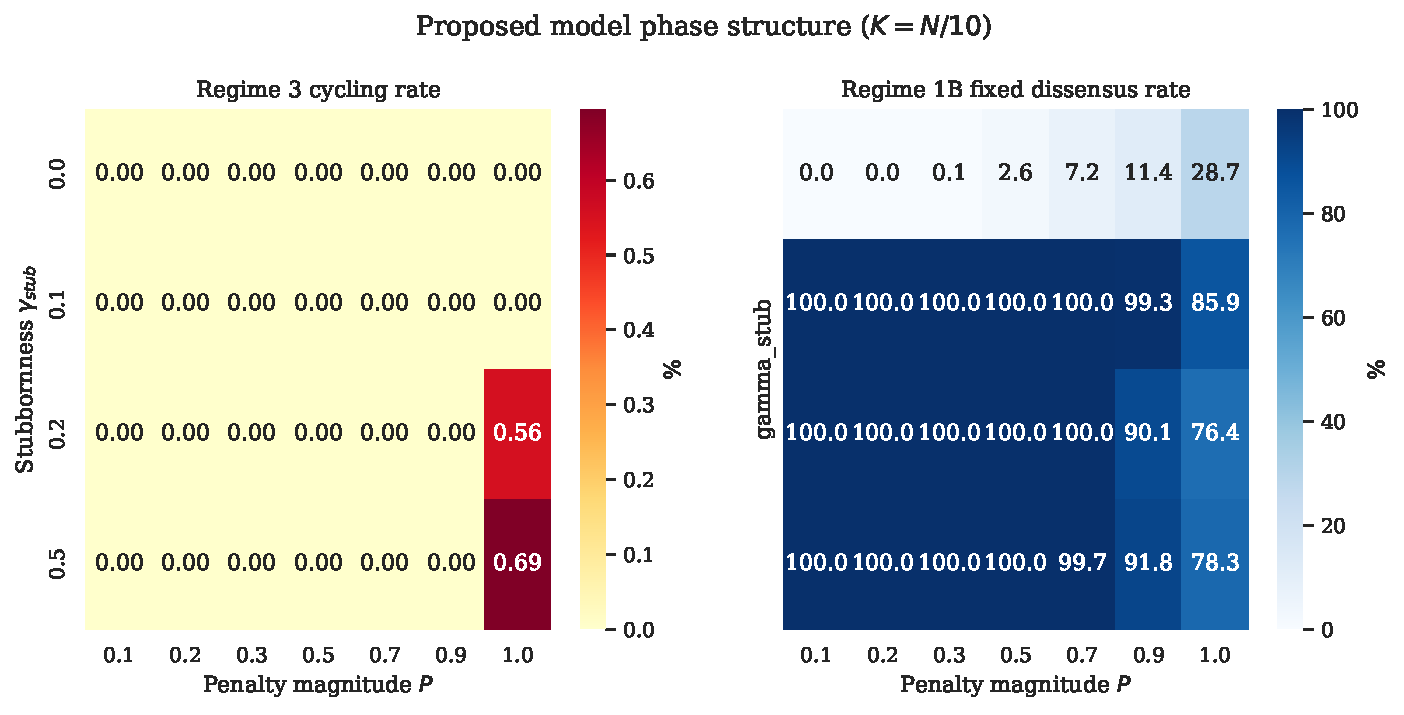
\includegraphics[width=\linewidth]{figures/fig03_phase_heatmaps.pdf}
  \caption{Empirical phase portraits for the proposed model with $K=N/10$. Left: Regime~3 cycling rate. Right: Regime~1B fixed dissensus rate.}
  \label{fig:phase-heatmaps}
\end{figure}

\begin{figure}[htbp]
  \centering
  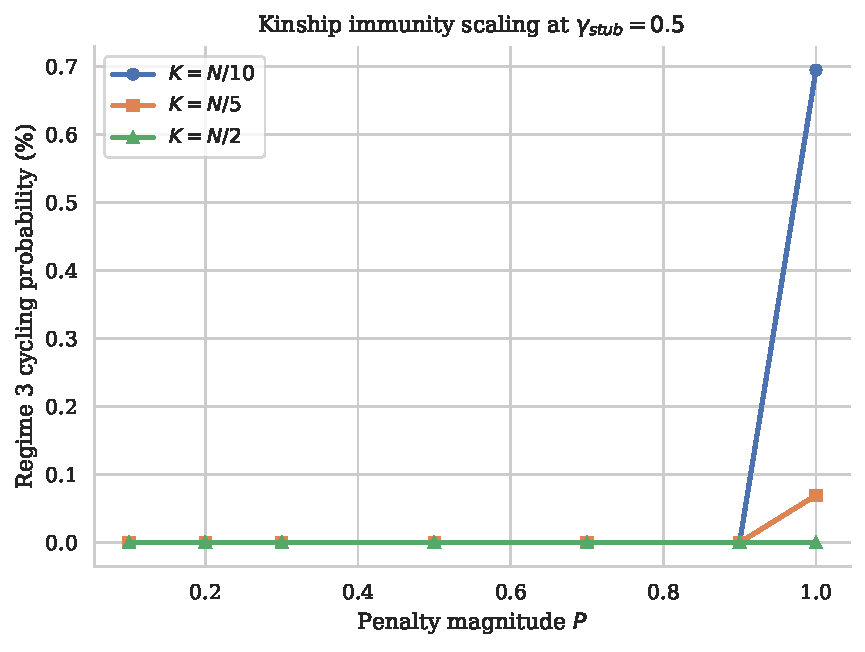
\includegraphics[width=0.78\linewidth]{figures/fig04_kinship_scaling.pdf}
  \caption{Kinship immunity scaling curves at $\gamma_{stub}=0.5$.}
  \label{fig:kinship}
\end{figure}

\begin{figure}[htbp]
  \centering
  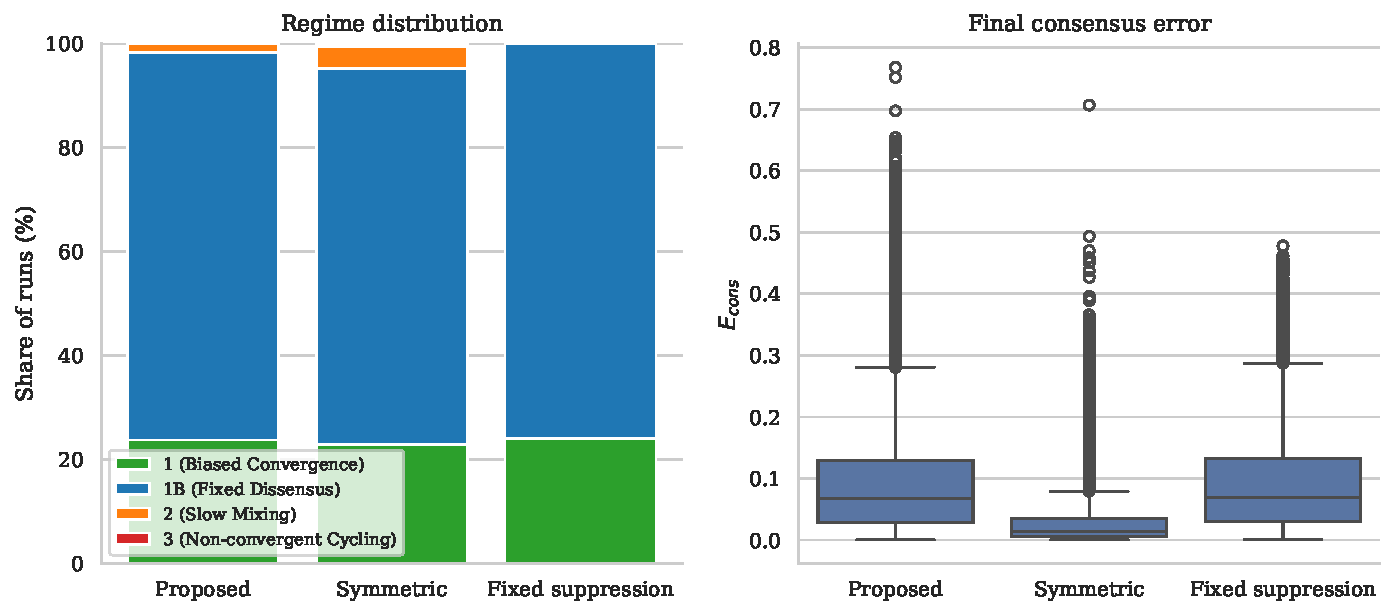
\includegraphics[width=\linewidth]{figures/fig05_ablation.pdf}
  \caption{Ablation comparison across proposed, symmetric, and fixed-suppression models.}
  \label{fig:ablation}
\end{figure}

\begin{figure}[htbp]
  \centering
  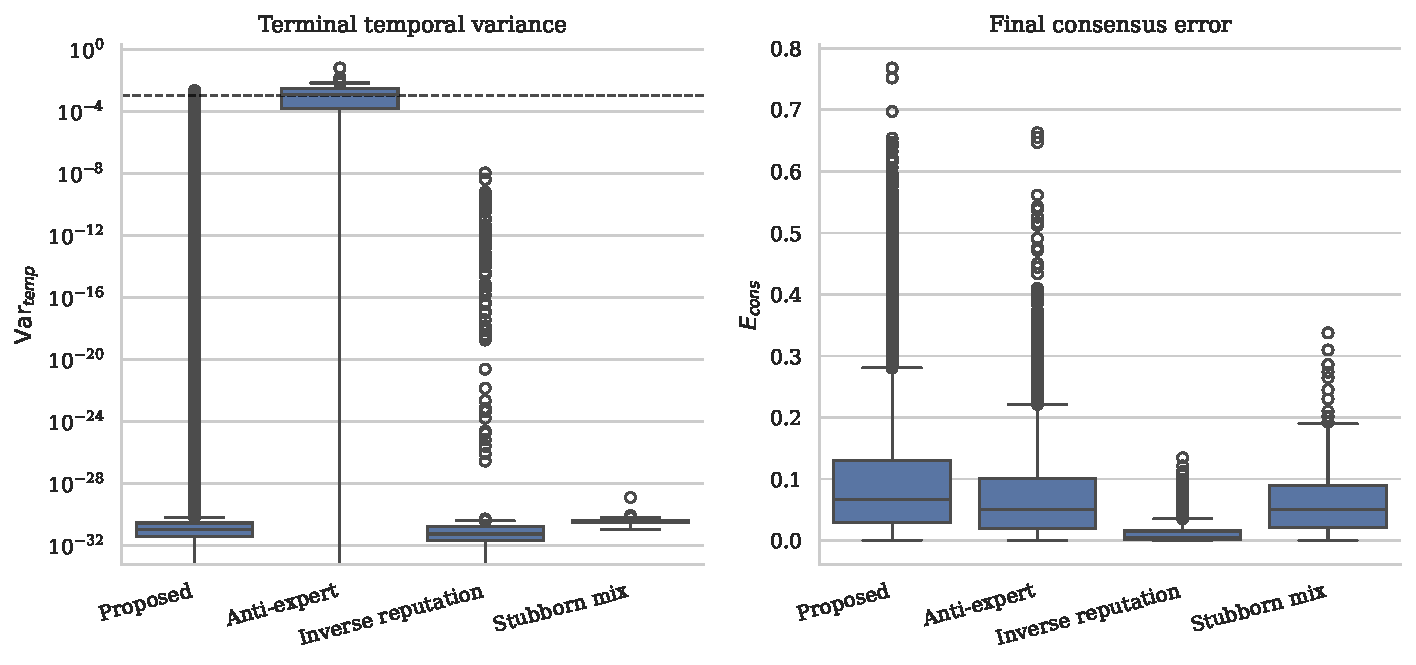
\includegraphics[width=\linewidth]{figures/fig06_baselines.pdf}
  \caption{Baseline comparison of temporal variance and consensus error.}
  \label{fig:baselines}
\end{figure}

\begin{table}[htbp]
  \centering
  \caption{Cross-model performance summary across validated simulation runs.}
  \label{tab:cross-model}
  \begin{tabular}{lrrrrrr}
    \toprule
    Model & Runs & R1 (\%) & R1B (\%) & R2 (\%) & R3 (\%) & $\bar{E}_{cons}$ \\
    \midrule
    Proposed & 122{,}880 & 23.76 & 74.56 & 1.67 & 0.02 & 0.0924 \\
    Symmetric & 122{,}880 & 22.96 & 72.47 & 4.05 & 0.52 & 0.0259 \\
    Fixed suppression & 122{,}880 & 24.02 & 75.98 & 0.00 & 0.00 & 0.0915 \\
    Anti-expert & 1{,}920 & 20.89 & 2.19 & 22.40 & 54.53 & 0.0766 \\
    Inverse reputation & 1{,}920 & 25.00 & 75.00 & 0.00 & 0.00 & 0.0119 \\
    Stubborn mix & 480 & 0.00 & 100.00 & 0.00 & 0.00 & 0.0620 \\
    \bottomrule
  \end{tabular}
\end{table}

\section{8. Conclusion}
This study formalizes the sociological phenomenon of status-based peer penalization within a distributed consensus framework\cite{degroot1974reaching}. By operationalizing "tall poppy syndrome" as an endogenous, state-dependent weight suppression operator, this work provides a mathematical framework for analyzing how social leveling pressures and anti-excellence behaviors disrupt decentralized agreement\cite{degroot1974reaching}. Because dynamic row normalization strictly preserves row-stochasticity at every time step, agent estimates remain confined within the convex hull of initial private estimates, ruling out unbounded arithmetic divergence\cite{degroot1974reaching}. The appropriate analytical framework for this model is the theory of switched affine discrete-time dynamical systems: the peer interaction matrix acts as a contraction mapping on the disagreement space, while cognitive anchoring continuously re-injects initial state dispersion into the network\cite{acemoglu2013opinion,hajnal1958weak}.

Theoretical analysis and extensive computational simulations across 372,960 verified network evaluations demonstrate that the interaction between leveling penalties and cognitive stubbornness partitions network dynamics into four distinct stability regimes\cite{degroot1974reaching,acemoglu2013opinion}:

Biased Convergence (Regime 1): Under weak suppression ($P < 0.3$) or in the absence of cognitive anchoring ($\gamma_{stub} = 0$), the network contracts to a uniform consensus\cite{degroot1974reaching,acemoglu2013opinion}. However, this agreement is systematically biased away from the true mean because unpenalized lower-performing agents are over-weighted during intermediate updates\cite{degroot1974reaching}. When $\gamma_{stub} = 0$, outliers are inevitably assimilated into the group average, permanently erasing superior information\cite{degroot1974reaching}.

Fixed Dissensus (Regime 1B): Under moderate-to-severe penalties combined with partial stubbornness ($\gamma_{stub} > 0$), peer influence weights stabilize, and opinion dynamics freeze into a stationary, non-consensus equilibrium\cite{acemoglu2013opinion}. Agents maintain persistent, non-zero spatial variance while their temporal variance drops to zero ($\text{Var}_{temp} \approx 0$)\cite{acemoglu2013opinion}. Cognitive anchoring establishes an irreducible floor that arrests downward assimilation without inducing periodic motion\cite{degroot1974reaching,acemoglu2013opinion}.

Slow Mixing (Regime 2): Near transition boundaries, state trajectories exhibit prolonged relaxation transients\cite{degroot1974reaching,acemoglu2013opinion}. Interaction weights chatter across the state-dependent switching boundary, producing slow algebraic mixing without settling into clean periodic orbits\cite{acemoglu2013opinion,hajnal1958weak}.

Non-convergent Cycling (Regime 3): Under maximal suppression ($P = 1.0$) paired with cognitive stubbornness ($\gamma_{stub} > 0$), the network undergoes a border-collision bifurcation into a self-sustaining, bounded limit cycle\cite{degroot1974reaching,acemoglu2013opinion,hajnal1958weak}. Accurate outliers are silenced, the collective drifts downward, the standardized deviation of the outliers normalizes as the group catches up, their broadcast influence is restored, they pull the group upward, and the penalty reactivates\cite{degroot1974reaching}. This periodic non-convergence occurs in positive row-stochastic networks without requiring negative edge weights (signed graphs) or absolute zealots\cite{acemoglu2013opinion,hajnal1958weak}.

The empirical data establishes a structural immunity threshold: kinship clustering\cite{degroot1974reaching}. When a mutually exempt in-group reaches a critical mass of the population ($K \ge N/5$), the incidence of non-convergent limit cycles drops to zero across all parameter configurations\cite{degroot1974reaching,acemoglu2013opinion}. Internal in-group edges remain unpenalized, preserving an invariant scrambling core that maintains communication throughput across the network and forces the collective into stationary dissensus or biased consensus\cite{degroot1974reaching,acemoglu2013opinion,hajnal1958weak}.

Ablation experiments confirm the structural drivers of this instability\cite{degroot1974reaching}. Symmetric penalization—suppressing both positive and negative outliers—acts as a coercive leveling clamp that minimizes estimation error relative to initial ground truth, but increases limit-cycle susceptibility by an order of magnitude (0.52% cycling compared to 0.02% in the directional model) by severing both tails of the communication graph simultaneously\cite{degroot1974reaching,acemoglu2013opinion}. The fixed suppression ablation confirms that sustained cycling requires active, state-dependent temporal feedback; locking weights at $t = 0$ collapses the system into a static linear model where cycling is mathematically impossible\cite{degroot1974reaching,acemoglu2013opinion}.

Benchmarking against established algorithms demonstrates the distinction between organic social leveling and algorithmic artifacts\cite{degroot1974reaching}. Rolling inverse-variance models (anti-expert weighting) exhibit catastrophic failure rates (54.53% cycling), triggered by exploding weights as opinions converge toward machine precision\cite{degroot1974reaching,acemoglu2013opinion}. The tall poppy operator avoids this numerical artifact through instantaneous, scale-invariant normalization, demonstrating that the observed limit cycles are organic mathematical properties of the tension between individual cognitive anchoring and collective peer leveling\cite{degroot1974reaching,acemoglu2013opinion}.

These findings suggest several avenues for future research:

Continuous-Time and Filippov Inclusions: Formulating the state-dependent penalty as a continuous-time hybrid system would allow the application of Filippov differential inclusions and Clarke generalized gradients to rigorously analyze sliding-mode behavior across the switching surface $\mathcal{S} = \{x : D_i(x) = \theta\}$\cite{hajnal1958weak}.

Asynchronous Consensus Protocols: Investigating this mechanism under randomized gossip or asynchronous updates would test whether sequential edge activations dampen or exacerbate border-collision limit cycles\cite{acemoglu2013opinion,hajnal1958weak}.

Multi-Layer and Multiplex Networks: Extending status penalties to multi-layer graphs would determine whether cross-platform communication channels mitigate ergodicity failure, allowing agents who face status leveling in one topical layer to maintain unpenalized influence in another\cite{degroot1974reaching}.

Time-Delayed Information Processing: Incorporating lagged communication channels would model the temporal delay inherent in social reputation tracking, potentially expanding the parameter boundaries under which self-sustaining limit cycles emerge\cite{degroot1974reaching,hajnal1958weak}.

By bridging non-homogeneous algebraic graph theory with empirical social psychology, this framework provides a rigorous foundation for identifying how decentralized peer sanctioning shapes the mathematical boundaries of consensus in human and artificial multi-agent systems\cite{degroot1974reaching}.



\section*{Data and Code Availability}
The simulation code, analysis scripts, and complete dataset (\texttt{full\_results\_v2.csv}) are available at
\url{https://github.com/advit-singh/influence-suppression-consensus-cycling}.

\bibliographystyle{plain}
\bibliography{references}

\end{document}
